\documentclass[12pt,a4paper]{styles/report}
\usepackage{mathtext}
\usepackage[T2A]{fontenc}
\usepackage[utf8x]{inputenc}
\usepackage[english, russian]{babel}
\usepackage{textcase}
%\usepackage[labelfont=bf]{caption}
%\usepackage{threeparttable}

\usepackage{color}

\definecolor{pblue}{rgb}{0.13,0.13,1}
\definecolor{pgreen}{rgb}{0,0.5,0}
\definecolor{pred}{rgb}{0.9,0,0}
\definecolor{pgrey}{rgb}{0.46,0.45,0.48}

\usepackage{listings}
\lstset{language=Java,
	basicstyle=\tiny,
	showspaces=false,
	showtabs=false,
	breaklines=true,
	showstringspaces=false,
	breakatwhitespace=true,
	commentstyle=\color{pgreen},
	keywordstyle=\color{pblue},
	stringstyle=\color{pred},
	basicstyle=\ttfamily,
	moredelim=[il][\textcolor{pgrey}]{$$},
	moredelim=[is][\textcolor{pgrey}]{\%\%}{\%\%}
}


\include{styles/preable}



%\bibident=0pt

\begin{document}
	
\renewcommand\contentsname{СОДЕРЖАНИЕ}
\renewcommand{\bibname}{БИБЛИОГРАФИЧЕСКИЙ СПИСОК}
\renewcommand\chaptername{ГЛАВА}
\renewcommand\figurename{Рисунок}
\renewcommand\tablename{Таблица}

\include{src/title_referat}

\newpage
\pagestyle{plain} \pagenumbering{arabic} \setcounter{page}{2}
\large \tableofcontents

\newpage
\chapter*{Перечень условных обозначений и сокращений}
\addcontentsline{toc}{chapter}{Перечень условных обозначений и сокращений} % in Content
В настоящей пояснительной записке применяются следующие термины, обозначения и сокращения.

НФ – Новая Физика.\\

СМ – Стандартная Модель.
ЛЭП – большой электрон-позитронного коллайдер.
ДЯ – Дрелл-Янга.
ATLAS (A Toroidal LHC ApparatuS) – один из четырёх основных экспе-риментов на Большом адронном коллайдере в Европейской организации ядерных исследований CERN в городе Женева (Швейцария).
SLC (Virtual Reality) – коллайдер сталкивающий электроны и позитроны каждый с энергией до 50 ГэВ.
БАК - Большой Адронный Коллайдер

\chapter*{ВВЕДЕНИЕ}
\addcontentsline{toc}{chapter}{ВВЕДЕНИЕ} % in Content
ыыыы

\chapter*{ОБЩАЯ ХАРАКТЕРИСТИКА РАБОТЫ}
\addcontentsline{toc}{chapter}{ОБЩАЯ ХАРАКТЕРИСТИКА РАБОТЫ} % in Content
\textbf{Связь работы с научными программами (проектами) и темами}\\

Диссертационная работа связана с тематикой НИР, выполняемых в рамках научно-исследовательского направления кафедры «Информационные технологии» Гомельского государственного технического университета им. П. О. Сухого.
Тема диссертации соответствует приоритетным направлениям
фундаментальных исследований в Республики Беларусь. Диссертационная
работа выполнялась в период с 2017 по 2019 годы в рамках отдельного
подзадания государственной программы научных исследований
«Конвергенция-2020», подзадание 2.1.05, номер гос. регистрации 20162284. Работа проводилась в рамках научно-исследовательских проектов 
кафедры «Информационные технологии» при сотрудничестве с ОИЯИ:  
\begin{enumerate}
	\item[--] «Нейросеть-ГО для GEMD» (договор с НИИ ЯП БГУ № 202/17(039/64)  
	от 25.07.2017 г.).
	\item[--] «Разработка новых алгоритмов реконструкции треков элементарных  
	частиц и проектирование программного средства для реализации методов  
	глубокого обучения в обработке экспериментальной информации с современных  
	трековых детекторов физики высоких энергий» (договор с НИИ ЯП БГУ №  
	206/18 от 14.09.2018 г.);
\end{enumerate}\\

\vspace{16pt}

\textbf{Цель и задачи исследования}\\

Целью работы является создание системы, определяющей возможность рождения нового резонанса нейтрального спина 1 (${Z}^{\prime}$) 
из доступных данных групп \textit{ATLAS} для ${W}^{+}{W}^{-}$ распадов. В качестве результатов работы будут получены 
ограничения на соответствующие $Z$-${Z}^{\prime}$-коэффициенты смешивания и на массу $M_{Z^\prime}$.

Для достижения поставленной цели были поставлены следующие задачи:

\begin{enumerate}
	\item[--] изучить процесс рождения ${Z}^{\prime}$-бозонов и распад ${W}^{+}{W}^{-}$ бозонов на Большом адронном коллайдере;
	
	\item[--] разработать имитационную модель процесса рождения ${Z}^{\prime}$-бозонов в протон-протонных столкновениях с учетом эффектов $Z$-${Z}^{\prime}$ смешивания;
	
	\item[--] выполнить разработку программного обеспечения для имитационного моделирования и оценки ограничений на соответствующие $Z$-${Z}^{\prime}$ параметры смешивания и на массу $M_{Z^\prime}$.
	
\end{enumerate}

Изучение появления электрослабых бозонов дает мощную проверку спонтанного нарушения 
калибровочной симметрии стандартной модели и может быть использовано для поиска новых явлений за пределами стандартной модели. 
Дополнительные нейтральные векторные бозоны ${Z}^{\prime}$, распадающиеся на заряженные пары калибровочных векторных бозонов ${W}^{+}{W}^{-}$, 
прогнозируются во многих сценариях новой физики, включая модели с расширенным калибровочным сектором.
\\

\textbf{Научная новизна}\\

Научная новизна работы заключается в том, что впервые получены ограничения на угл смешивания ${Z}^{\prime}$-бозонов в
процессе рождения ${W}^{+}$${W}^{-}$ пар в протон-протонных столкновениях для значений светимости 1000 фб${}^{−1}$ и 3000 фб${}^{−1}$ на Большом адронном коллайдере, а также создан программный модуль, позволяющий выполнять: имитационное моделирование рождения ${Z}^{\prime}$ в процессе ${W}^{+}{W}^{-}$
на Большом адронном коллайдере с учётом эффектов $Z$-${Z}^{\prime}$ смешивания.
\\

\textbf{Положения, выносимые на защиту}\\

Автором защищаются:
\begin{enumerate}
	\item[--] имитационная модель процесса рождения ${Z}^{\prime}$-бозонов в протон-протонных столкновениях с последующим распадом на пару ${W}^{+}{W}^{-}$ бозонов, отличающаяся от известных моделей учетом эффектов $Z$-${Z}^{\prime}$ смешивания;
	
	\item[--] программный модуль для имитационного моделирования процесса
	рождения ${Z}^{\prime}$-бозонов в протон-протонных столкновениях с учетом эффектов $Z$-${Z}^{\prime}$ смешивания в условиях эксперимента \textit{ATLAS} на Большом адронном коллайдере, отличающуюся от существующих тем, что программный модуль собран в \textit{Docker} образ позволяющий быстро проводить имитационное моделирование без установки необходимых программных средств;
	
	\item[--] оценки ограничений на углы смешивания ${Z}^{\prime}$-бозонов в
	процессе рождения ${W}^{+}$${W}^{-}$ пар в протон-протонных столкновениях
	в условиях экспериментов на Большом адронном коллайдере, рассчитаные для интегральной светимости 1000 фб${}^{−1}$ и 3000 фб${}^{−1}$, которые составили  ${10}^{-4}$ и $6\times{10}^{-5}$, соответственно, и существенно превышают существующие экспериментальные ограничения.
	
\end{enumerate}
\vspace{2cm}

\textbf{Личный вклад соискателя}\\

Содержание диссертации целиком и полностью отображает личный вклад соискателя. Определение целей и задач исследования, обобщение полученных результатов проводилось совместно с научным руководителем К.С. Курочкой.\\

%Диссертация прошла проверку на плагиат в системе обнаружения текстовых заимствований с результатом 80\% оригинальности.
\\

\textbf{Апробация результатов диссертации}\\

Результаты работы докладывались на V Международной конференции <<Инновации в современной науке>> (Киев, июнь 2019 г.).
\\

\textbf{Опубликованность результатов диссертации}\\

Результаты диссертационных исследований, связанных с измерением процесса рождения ${W}^{+}{W}^{-}$ пар в протон-протонных столкновениях и получены экспериментальные ограничения на угол смешивания ${Z}^{\prime}$-бозонов направлены в печать в рамках V Международной конференции <<Инновации в современной науке>> [1-A].
\\

\textbf{Структура и объем диссертации}\\

Диссертационная работа состоит из введения, четырёх глав, заключения и библиографического списка. Объем диссертации – 79 листов, включая 1 приложение и 20 иллюстраций. Библиографический список содержит 23 наименований, так же 1 публикацию соискателя.


\chapter{Анализ программ моделирования процессов столкновения элементарных частиц при высоких энергиях}
\input{src/2-2-Zprime}

Современное программное обеспечение для обработки медицинских изображений

\section{Обзор генератора <<PYTHIA>>}
\textit{PYTHIA} это программа для генерации событий физики
высоких энергий, т.е., для описания столкновений таких
высокоэнергетических элементарных частиц, как электрон,
позитрон, протон и антипротон в различных комбинациях.
Информация для моделирования взята по большей части из
собственных исследований в ЦЕРН, однако, много формул и
другой информации почерпнуто из научной литературы~\cite{review-pythia}.

С 1997 года по нынешнее время использовалась версия
этого Монте-Карло генератора, написанная в \textit{FORTRAN77}
(текущая версия 6.4). Сейчас программа переписана в \textit{С++}
(версия 8.1), однако, до тех пор, пока не осуществлен
перевод всех возможностей, обе версии используются и
поддерживаются одновременно.


Назначение генераторов физических событий:
\begin{itemize}
	\item[--] Дают физикам представление о типе событий, которые
	они надеются увидеть, и об их скорости набора;
	\item[--] Помогают в планировании новых детекторных установок,
	то есть, оптимизировать их характеристики для изучения
	интересующих сценариев физических событий в рамках
	существующих ограничений;
	\item[--] Являются инструментом для проработки стратегии
	анализа данных (оптимизации отношения “сигнал/шум”);
	\item[--] Используются в качестве метода оценки коррекций на
	геометрические и кинематические ограничения области
	чувствительности (acceptance) детекторов;
	\item[--] Используются в качестве удобной рабочей оболочки для
	интерпретации наблюдаемых феноменов в терминах
	Стандартной Модели.
\end{itemize}

Квантовая механика вносит концепцию случайности в
поведение физических процессов. Достоинством
генераторов событий (\textit{event generators}) является то, что эта
случайность может быть смоделирована при помощи метода
Монте-Карло. Сущность метода заключается в том, что, вопервых подразумевается наличие генератора
псевдослучайных чисел, т.е. функции, которая при вызове
возвращает число R в пределах от 0 до 1, при этом
распределение R является плоским, и с достаточной
точностью значения \textit{R} являются нескоррелированными~\cite{review-pythia}.
Затем эти значения \textit{R} используется для розыгрыша сценария
конкретного цикла события (выбор конкретного значения
для различных известных распределений величин, выбор
времени распада и т.п.) Разыграв статистически достаточное
количество событий, мы можем построить интересующие
нас распределения (например, диапазон энергий для
продуктов интересующего механизма реакции).
Что касается упомянутых известных распределений,
то, например, дифференциальное сечение реакции
рассчитывается из кинематических соотношений при
введении матричного элемента (известного, либо
предложенного теоретиками исходя из перспективных
моделей), для учета высших порядков КХД вводится
значение дополнительного параметра (K-множителя).
Следует заметить, что при генерации значительного
числа событий (миллионов), становится актуальной
проблема скоррелированости псевдослучайных чисел, и
вместо встроенных в \textit{C++ Random} генераторов приходится
применять специально созданные программы.


С точки зрения описания физики событий полная
процедура генерации события разделяется на 3 стадии:

\begin{enumerate}
	\item Генерация «процесса», который определяет природу
	события. Зачастую это могут быть «жесткие процессы»,
	такие как $gg \rightarrow {h}^{0} \rightarrow ZZ \rightarrow {m}^{+}{m}^{-}{qq}_{bar}$ (а также другие
	процессы), которые могут быть просчитаны в рамках
	теории малых возмущений.

	\item Генерация всех подчиненных процессов на партонном
	уровне, включая гамма-излучение, многократное партонные
	взаимодействия и структуру непровзаимодействовавшего
	пучка. Такие феномены приблизительно описываются
	теорией малых возмущений, однако непертурбативные
	поправки уже существенны.
	\item Адронизация этой партонной конфигурации
	(фрагментация струй, распады нестабильных частиц).
	Только феноменологическое описание
\end{enumerate}

Этим стадиям отвечают три класса \textit{ProcessLevel},
\textit{PartonLevel} и \textit{HaronLevel}, соответственно. Классы: \textit{Event}
(члены класса \textit{process} и \textit{event}), \textit{BeamParticles}, база данных
\textit{Settings}

С точки зрения технического устройства,
взаимодействия пользователя и генератора проявляется в
трех фазах:


\begin{enumerate}
	\item Инициализация, когда формулируется задание.
	\item Генерация индивидуального события (цикл события).
	\item Вывод окончательной статистики.
\end{enumerate}

Программа содержит теорию и модели для ряда
аспектов физики, включая так называемые мягкие и жесткие
взаимодействия, распределения партонов, партонные струи
начального и конечного состояний, многократные
партонные взаимодействия, фрагментацию и распады~\cite{review-pythia}.

Встроенные \textit{C++} методы программы обеспечивают
доступ к информации как об отдельной частице либо
процессе на любом этапе розыгрыша события, так и о
событии в целом. Встроенные средства вывода позволяют
получить статистическую информацию и гистограммы в
виде ASCII кода (который можно сохранить в файл для
дальнейшего использования).

Пакет \textit{Pythia} является компактной (\textit{5 Мб} )
независимой программой, поэтому несложно скачать и
установить себе собственную локальную версию. Для этого
архив установочный код (в 2011 году был \textit{8145.tgz}) можно
скачать с сайта разработчика или с кафедрального сайта~\cite{review-pythia}.
Затем его нужно распаковать (команда \textit{tar -xzf 8145.tgz})
и скомпилировать (команда make в распакованной корневой
директории, занимает ~2 минут на \textit{lx}).

Быстрее всего начать работу с обучающими и своими
первыми скриптами в поддиректории examples. В пакеты \textit{Pythia} можно создать такой объемный процесс, как генератор
моделирющий столкновение барионов на \textit{LHC} с рождением
топ-кварков. Так же в на сайте разработчиков бибилиотеки есть руководство в котором описываются возможности по настройке
свойств процессов и получения информации (например,
можно сделать бозон ${Z}^0$ стабильной частицей инструкцией \textit{pythia.readString("23:onMode=off")}). 

%http://lib.sinp.msu.ru/static/tutorials/141_Leontiev_Zadahi_2011.pdf
\section{Обзор генератора <<Powheg-Box>>}
Возмущающие вычисления КХД следующего порядка (NLO), а также ливень Монте-Карло
(SMC) программы являются фундаментальными инструментами современной феноменологии физики элементарных частиц. В частности, программы SMC включают описание общего адронного столкновения высокой энергии
процесс, начиная от столкновения между составляющими и развития партонного ливня, что
увеличивает количество частиц в конечном состоянии за счет сильно упорядоченных последующих выбросов.
В конце концов, интерфейс с феноменологической моделью адронизации позволяет сравнивать
с экспериментальными данными. По этим причинам они обычно используются экспериментаторами для
моделировать сигнальные и фоновые процессы в физических поисках. Тем не менее, спрос на
лучшие и лучшие прогнозы из экспериментов с высокой энергией требуют повышения точности
существующих SMC, включая исправления NLO. Метод MC @ NLO [1] сначала показал, как
достичь точности NLO для инклюзивных количеств, реализуя жесткий подпроцесс в NLO и
развитие ливней в ведущем логарифмическом приближении, избегая двойного счета
излучение. Таким образом можно достичь преимуществ обоих подходов: генерация исключительных конечных состояний
SMC и точность расчетов NLO.

\section{Обзор генератора <<Sherpa>>}
Наиболее яркими примерами генераторов событий являются очень успешные, хорошо отлаженные программы
PYTHIA [1] и HERWIG [2]. Они были построены за последние десятилетия наряду с экспериментальными открытиями, и большинство особенностей, видимых в прошлых и настоящих экспериментах, могут быть описаны
ими. Тем не менее, необходимость в более высокой точности для решения задач новых энергетических масштабов происходящих
на \textit{LHC}, сложность конечных состояний в этих масштабах, необходимость обслуживания и желание легкой возможности реализовать новые физические модели, требовалось переписать эти пакеты на современном языке программирования, обеспечивающем более высокий уровень модульности. Объектно-ориентированные рамки отвечают последним
требования и в связи с предпочтениями сообщества к \textit{С++}, новое поколение генераторов событий
построено на этом языке программирования. Это привело к улучшению повторных реализаций в форме
программ \textit{PYTHIA 8} [3] и \textit{HERWIG ++} [4] - преемники версий написаных на \textit{Fortran}, упомянутых выше
и к созданию генератора событий \textit{SHERPA} [5].
В связи с этим в последнее десятилетие стали доступны пакеты для расчетов с опережающим порядком. Яркими примерами являются \textit{MCFM} [6] и \textit{NLOJET ++} [7]. Соответствующие методы реализованы, например, в \textit{MC@NLO} [10], который основан
на фортранской версии \textit{HERWIG}, в \textit{HERWIG ++} [11] и в некоторых более специализированных программах [12].
Тем не менее, полные расчеты следующего за ведущим порядком, лежащие в основе этих новых методов, очень сложны, и до сегодняшнего дня контролируются только процессы с пятью внешними ветвями. Но
с другой стороны, многие важные экспериментальные сигнатуры зависят от конечных состояний с более высокой кратностью, что
инициировало существенную деятельность по совершенствованию методов и инструментов с точностью на уровне множества ветвей, так что
теперь доступно несколько пакетов, которые могут вычислять соответствующие сечения и генерировать события
полностью автоматизированным способм. Наиболее яркими примерами являются \textit{ALPGEN} [13], \textit{CompHEP} / \textit{CalcHEP} [14],
\textit{HELAC-PHEGAS} [15], \textit{MADGRAPH} [16], \textit{WHIZARD} [17] и \textit{AMEGIC ++} [18]. В настоящее время только библиотека \textit{AMEGIC ++} реализует данный функционал и встроенная в полноценный генератор событий, а именно в среду \textit{SHERPA}. Чтобы
преобразовать многочастичные события на уровне партонов, которые предоставляются этими инструментами в ведущем порядке, в
события уровня адронов, было разработано несколько алгоритмов, все из которых направлены на сохранение логарифмической
точности партонного потока и дополнения его точным результатом возмущающего ведущего порядка для
учитывания кратности струи.

\textit{SHERPA} [5] является аббревиатурой от «“Simulation of High Energy Reactions of Particles». Программа является
полная структура генерации событий, которая была построена с нуля и полностью написана в
современный объектно-ориентированный язык программирования \textit{C++}

Построение SHERPA осуществлялось способом, в значительной степени определяемым следующими тремя парадигмами:


% https://arxiv.org/format/0811.4622

\section{Постановка задачи на диссертационное исследование}

\chapter{РАЗРАБОТКА АЛГОРИТМОВ И ТЕХНОЛОГИЙ РЕШЕНИЯ ПОСТАВЛЕННОЙ ЗАДАЧИ}
\section{Рождения $Z^\prime$ - бозонов в протон-протонных столкновениях с учетом эффектов $Z$ - $Z^\prime$ смешивания}
Многие сценарии Новой Физики (НФ) отличной от Стандратной Модели (СМ)~\cite{2part-1}, включая модель суперпозиций и левую-правую симметричную модель, предсказывают существование новых нейтральных и заряженных калибровочных бозонов, которые могут быть найдены на текущих или будущих коллайдерах. Поиск нового нейтрального $Z^\prime$ и заряженного $W^\prime$ калибровочных бозонов является важным аспектом экспереметально-физических программ на колладерах больших энергий. В этой работе сконцентрировано внимание на первом бозоне.

Предоставленные лимиты большого адронного коллайдера и виртуальные эффекты ЛЭП, через интерференцию или смешивания с $Z$ бозонами, подразумевает что любые $Z^\prime$ бозоны горазда тяжелее и менее смешиваются с $Z$ бозонами. В зависимости от рассматриваемой теоретической модели $Z$ массы порядка 4,5 ТэВ~\cite{2part-pankov} и $Z-Z^\prime$ углов смешивания на уровне нескольких градусов исключены~\cite{sirunyan:2017}. Угол смешивания сильно ограничен очень высокоточными экспериментами на ЛЭП и \textit{SLC}. Они включают в себя измерения из формы линии \textit{Z}, из лептонных отношений ветвления, нормированных на общую адронную ширину затухания $Z$, а также от лептонных лево-правых асимметрий. $Z^\prime$, легче чем 5 ТэВ, может быть обнаружен на БАК~\cite{sirunyan:2017} c $\sqrt{s} = 14 $ ТэВ в процессе Дрелл-Янга (ДЯ) $pp \rightarrow Z^\prime \rightarrow l^+l^- + X$, где $l=e,\mu$.

После открытия $Z^\prime$-бозона на БАК через процесс ДЯ, необходимо произвести некоторую диагностику связей и смешивания $Z$-$Z^\prime$, чтобы идентифицировать основную теоретическую структуру. В настоящей работе исследуются данные \textit{ATLAS}~\cite{main-book} и \textit{CMS} в канале дибозона.

\begin{equation} \label{eq:1}
pp \rightarrow W^+W^- + X
\end{equation}

Для поиска \textit{Z}-бозона, который возникает, например, в популярной модели с расширенным калибровочным сектором~\ref{eq:1}. Анализ основан на данных о столкновениях $pp$ при энергии центра масс $\sqrt{s} = 13 $ собранных группами \textit{ATLAS}~\cite{main-book} и \textit{CMS} на БАК. В частности, данные используются для поиска $Z$-$Z^\prime$ смешивание. На \textit{ATLAS} события $W^+W^-$ реконструируются через их полулептонные распады $W$, где один $W$-бозон распадается на заряженный лептон ($l=e,\mu$) и нейтрино, а другой на две струи, тогда как на CMS $W$-бозон адронически распадается на две восстановленные струи. 

Процесс рождения пары $W^-W^+$-бозонов~\ref{eq:1} важен для изучения электрослабой калибровочной симметрии. Общие свойства слабых калибровочных бозонов тесно связаны с нарушением электрослабой симметрии и структуры калибровочного сектора, как и существование и структура трилинейных связей. Кроме того, канал распада дибозонов $Z^\prime$ исследует толщину калибровочной связи между новым и калибровочными бозонами стандартной модели. Кроме того, сила связи очень влияет на элементы распада и естественную ширину такого нового калибровочного бозона. Таким образом, детальное рассмотрение процесса~\ref{eq:1} с высокой точностью проверяет калибровочный сектор СM и может пролить свет на бозоны, которые могут появиться за пределами СМ. Здесь мы рассмотрим возможность наблюдения $Z^\prime$-бозона в $W^+W^-$ парного процесса на БАК, который в отличие от процесса ДЯ не является основным каналом поиска, но может помочь понять происхождение новых калибровочных бозонов.

Поиски тяжелого \textit{WW} резонанса были выполнены на Теватроне исследовательскими группами \textit{CDF} и \textit{D0}. Группа \textit{D0} изучала резонансное рождение дибозонов до 700 ГэВ в каналах распада $lvl^\prime v^\prime$ и $lvjj$~\cite{Krasnikov:2004}. Группа CDF также исследовала резонанс в $WW$ в канале распада $evjj$, что в результате привело к обнаружения нижних лимитов масс $Z^\prime$
и $W^\prime$-бозонов, за исключением масс превышающих 900 ГэВ, зависящих от параметра смешивания.

Исследования \textit{WW}-резонансов группами \textit{ATLAS} и \textit{CMS} с использованием, соответственно, полулептонных и адронных событий распада в $pp$ столкновениях при 13 ТэВ устанавливают массовые пределы 3 ТэВ для этих резонансов~\cite{nuclphys:weak}. 

В диссертационной работе изучается возможность рождения нового резонанса нейтрального спина 1 ($Z^\prime$) из доступных данных групп \textit{ATLAS} для $W^+W^-$ распадов. В качестве результатов работы будут получены ограничения на соответствующие $Z-Z^\prime$-коэффициенты смешивания и на массу $M_{Z^\prime}$.
Выполнено моделирование событий рождения $Z^\prime$ бозонов в процессе распада на фотонную пару и моделирование событий рождения гравитонов в процессе $lvl^\prime v^\prime$. Создано \textit{web}-приложение для демонстрации результатов вычисления.

Несмотря на впечатляющий успех в описании экспериментов, Стандартная модель не может считаться окончательной теорией элементарных частиц. У нее есть свои трудности. Физики уверены, что она должна быть частью некоторой более глубокой теории строения микромира, той частью, которая видна в экспериментах на коллайдерах при энергиях ниже примерно 1 ТэВ. Главная задача Большого адронного коллайдера — получить хотя бы первые намеки на то, что это за более глубокая теория.

Теоретики разработали большое число кандидатов на такую теорию. Все они, естественно, включают какие-то элементы, которые отсутствуют в Стандартной модели. Часто такие теории коллективно называют «Новая физика» или «За пределами Стандартной модели». На этой странице перечислены некоторые из активно изучаемых вариантов Новой физики~\cite{2part-1}.

\begin{figure}[h]
	\centering
	\includegraphics[width=\textwidth]{figures/hep-sm.png}
	\caption{Константы связи трех типов взаимодействий}
	\label{fig:fig01}
\end{figure}

Суперсимметрия -- это гипотетическая симметрия между фермионами и бозонами. Теории, использующие эту идею, оказываются удивительно мощными, и потому именно с суперсимметрией многие связывают надежды на открытие физики за пределами Стандартной модели. Однако до сих пор не было получено ни одного убедительного доказательства в пользу того, что суперсимметрия реализуется в нашем мире. Ее поиск является одной из главных задач Большого адронного коллайдера.

Константы связи трех взаимодействий частиц в микромире сходятся к одному значению, если имеющиеся сейчас данные экстраполировать в область очень высоких энергий. Это совпадение считается неслучайным и воспринимается физиками как намек на то, что все три взаимодействия при больших энергиях объединяются в одно.

В XIX веке физики обнаружили, что электричество и магнетизм — это две стороны одной медали, электромагнитного взаимодействия. Век спустя, при создании Стандартной модели, электромагнетизм и слабые ядерные силы были объединены в рамках единого электрослабого взаимодействия. (Точнее говоря, внутри электрослабого взаимодействия имеются по-прежнему две разные силы, а электромагнитное и слабое взаимодействия возникают как комбинации этих сил). Каждое такое объединение упрощало теорию, уменьшало количество введенных в нее «сущностей», переводило наше понимание микромира на новый уровень.

Сейчас физики имеют сразу несколько причин подозревать, что при очень высоких энергиях происходит объединение электрослабого и сильного взаимодействий (рисунок~\ref{fig:fig01}). Модели, использующие эту идею (так называемые Теории великого объединения) разрабатываются уже давно. В идеале хотелось бы, чтобы такая теория естественным образом объясняла, почему фундаментальных взаимодействий именно столько и именно с такими свойствами, а также имела четкие предсказания, доступные проверке в современных экспериментах~\cite{main-book2}.

При энергиях элементарных частиц, доступных на ускорителях, гравитация по-прежнему остается исключительно слабой, так что заметить ее проявления не удается. Однако ее сила растет с ростом энергии, и при энергиях столкновения порядка планковской она станет столь же важной, как и другие взаимодействия. В этом случае в полный рост встает исключительно сложный вопрос о том, как включить гравитацию в квантовое описание микромира. Поскольку гравитация в современной физике считается проявлением кривизны пространства-времени, успешная теория с сильной гравитацией должна описывать в рамках единого формализма не только все взаимодействия и всё вещество, но и структуру пространства-времени.

Одним из наиболее привлекательных путей решения этого вопроса является теория суперструн и ее дальнейшее развитие в виде теории бран и М-теории. В этих теориях считается, что фундаментальными объектами, существующими в многомерной вселенной, являются не точечные частицы, а протяженные объекты -- струны, мембраны и еще более многомерные образования. В этой теории были получены впечатляющие успехи при высоких энергиях, однако при попытке вывести свойства нашего низкоэнергетического мира из теории суперструн возникает обескураживающая неопределенность предсказаний.

Долгое время казалось, что проверка предсказаний теории суперструн лежит далеко за пределами возможностей человечества, поскольку речь идет об энергиях, на 15 порядков превышающих энергии современных ускорителей. Однако примерно 10 лет назад возникло новое направление развития теории, в котором гравитация становится сильной на энергиях порядка 1 ТэВ. Такая возможность возникает в том случае, если наш мир более чем трехмерный и если при этом новые дополнительные пространственные размерности достаточно протяженны: либо они бесконечны, либо свернуты в многомерные петельки размером много больше ядерного масштаба.

В этом случае на \textit{LHC} следует ожидать целый ряд совершенно замечательных эффектов, отсутствующих в Стандартной модели, например, рождение гравитонов, которые будут улетать из нашего мира в дополнительные измерения, и микроскопических черных дыр, тут же испаряющихся с испусканием множества обычных частиц. Будут также наблюдаться сильные отклонения от предсказаний Стандартной модели в столкновении обычных частиц. Стоит, впрочем, подчеркнуть, что пока нет никаких экспериментальных подтверждений того, что эта красивая гипотеза имеет отношение к нашему миру.

Все три перечисленные выше направления «Новой физики» опираются на глубокие теоретические гипотезы об устройстве нашего мира (суперсимметрия, единство сил, квантово-гравитационная вселенная). Однако кроме этих направлений теоретики также рассматривают разнообразные теории «статусом пониже». В этих теориях просто отмечается, что текущие экспериментальные данные не запрещают те или иные экзотические объекты или явления, и разрабатываются их следствия. Вот несколько примеров таких моделей разной степени экзотичности.

Неминимальные хиггсовские модели. Поскольку хиггсовские бозоны — единственные частицы Стандартной модели, до сих пор не открытые экспериментально, теоретики изучают самые разные варианты устройства этого сектора теории.
Новые поколения фермионов. Можно предположить, что кроме трех известных поколений кварков и лептонов существуют и другие поколения. Частицы из этих поколений должны быть очень тяжелыми, иначе бы их уже давно открыли в эксперименте.

Новые короткодействующие силы. В таких моделях предполагается, что в нашем мире есть и иные силовые взаимодействия, отличные от сильных, слабых и электромагнитных, но они настолько короткодействующие, что до сих пор никак не проявлялись в эксперименте. На Большом адронном коллайдере благодаря его рекордной энергии удается «прощупать» взаимодействия частиц на исключительно малых расстояниях (менее 10–19 метра), а значит, появляется шанс эти взаимодействия обнаружить. Они могут проявляться либо как рождение и распад частицы-переносчика новых сил (такие гипотетические частицы обозначают $Z^\prime$), либо как усиленное рассеяние частиц на большие углы.

\begin{figure}[h]
	\centering
	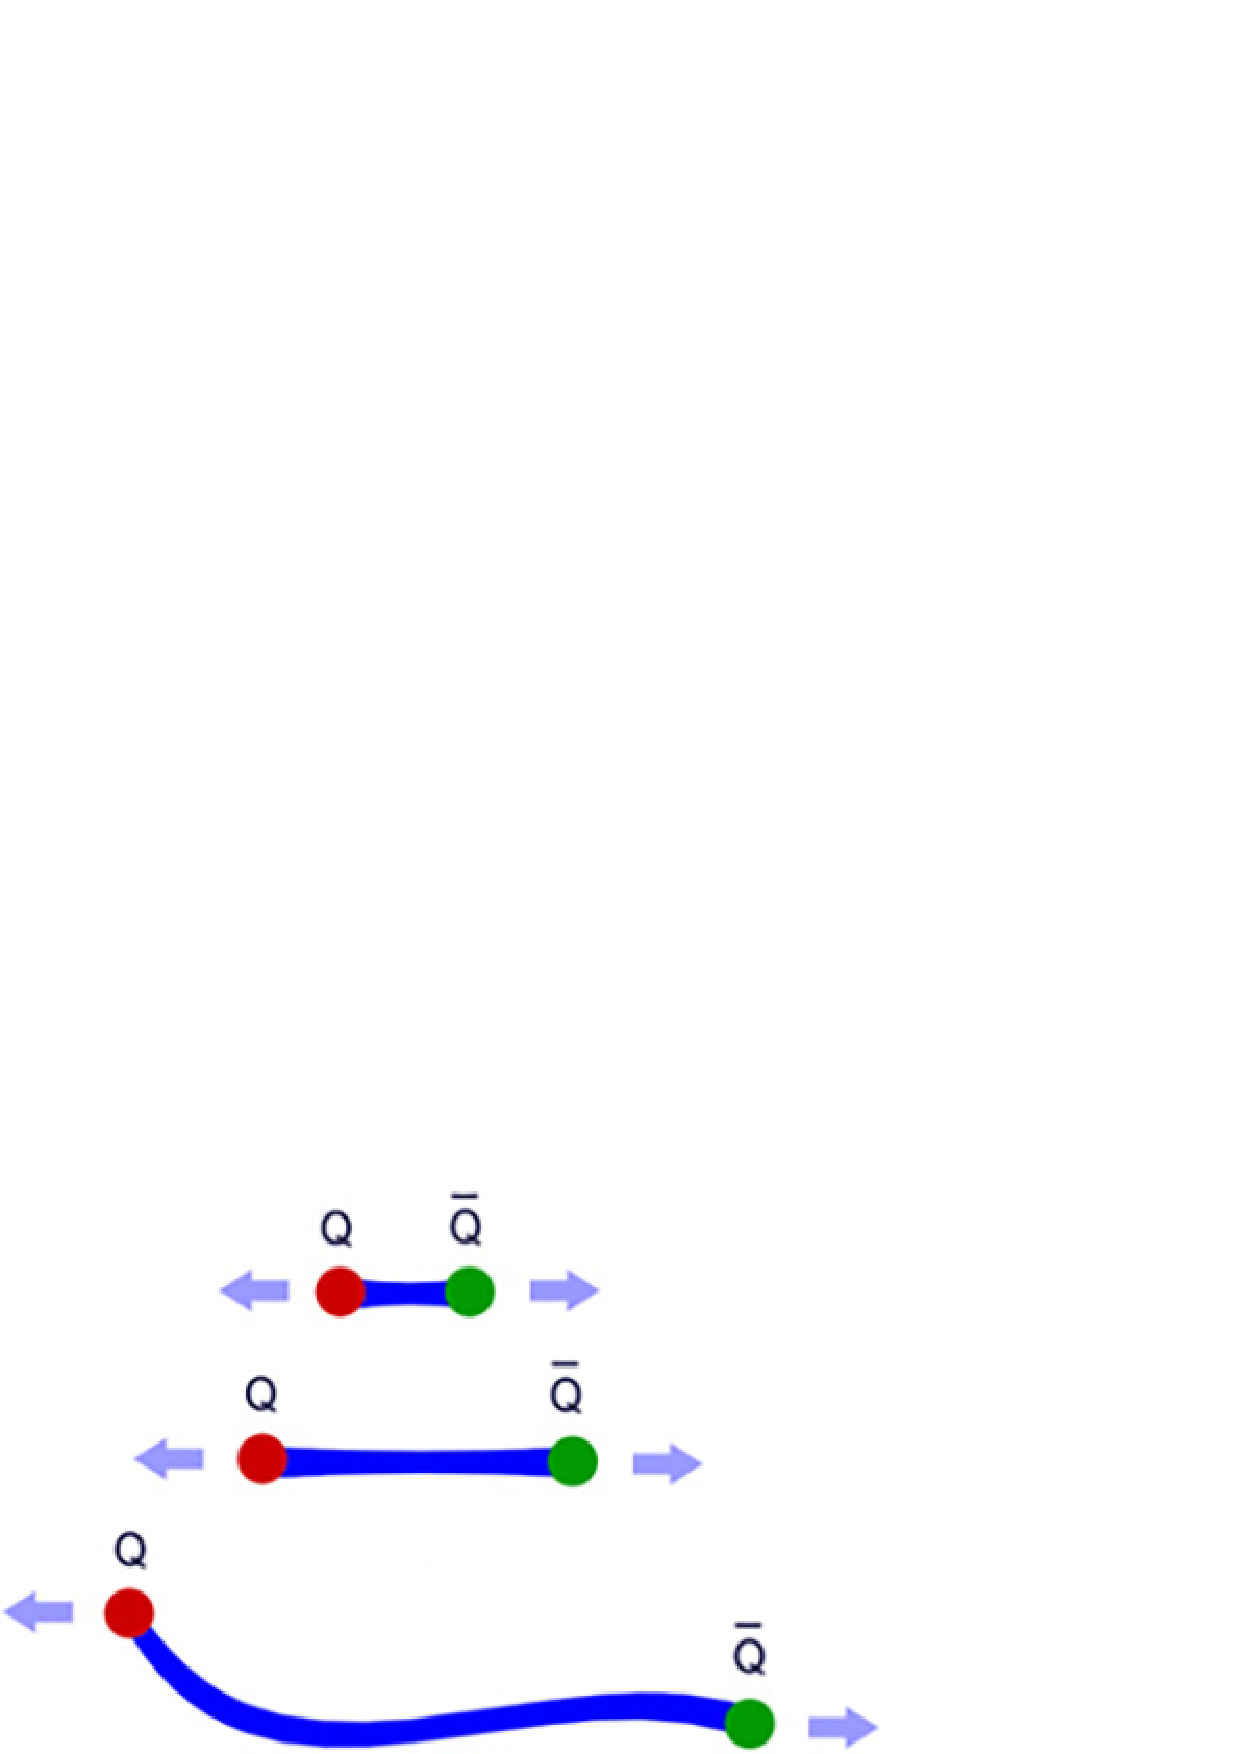
\includegraphics[width=\textwidth]{figures/quirk-antiquirk.jpg}
	\caption{Кварки}
	\label{fig:fig03}
\end{figure}

Лептокварки. В Стандартной модели и в подавляющем большинстве теорий Новой физики кварки и лептоны взаимодействуют друг с другом опосредованно, путем обмена квантами силовых полей. Однако можно представить себе возможность того, что кварки и лептоны исходно являлись фермионами одного типа и лишь потом расщепились на два разных сорта. В таком случае должны существовать новые тяжелые частицы — лептокварки, которые распадаются прямо на кварк и лептон. Подобные частицы встречаются в теориях Великого объединения.

Квирки. Одним из очень необычных и любопытных вариантов новых сил является гипотеза квирков (\textit{quirks}). Эта модель построена по типу обычного сильного взаимодействия: в ней предполагается, что существует новое силовое поле с конфайнментом и новые частицы, его чувствующие. Если частицы очень тяжелые, то между ними будут натягиваться длинные, даже макроскопические силовые струны, которые не смогут порваться (рисунок~\ref{fig:fig03}).

Слабое взаимодействие – короткодействующее фундаментальное взаимодействие между элементарными частицами, ответственное за бета-распад атомных ядер и медленные распады частиц. Слабое взаимодействие значительно слабее сильного и электромагнитного, но гораздо сильнее гравитационного. В слабом взаимодействии участвуют все фундаментальные фермионы (кварки и лептоны) и все адроны. Единственными частицами, которые участвуют только в слабом взаимодействии являются три типа нейтрино $v_e$, $v_\mu$, $v_\tau$ и их античастицы  антинейтрино $\bar{v_e}$,  антинейтрино $\bar{v_\mu}$,  антинейтрино $\bar{v_\tau}$. В нем не участвуют переносчики сильного, электромагнитного и гравитационного взаимодействий -- глюон, фотон и гравитон. В процессе слабого взаимодействия частицы обмениваются переносчиками слабого взаимодействия промежуточными (фундаментальными) бозонами: имеющими электрический заряд $W^±$ и нейтральным $Z$. Эти бозоны, в отличие от переносчиков остальных фундаментальных сил безмассовых глюона, фотона и гравитона, имеют огромные массы $m_W$ = 80.4 ГэВ/с~${}^2$ и $m_Z$ = 91.2 ГэВ/с${}^2$ (примерно как у атомов циркония или ниобия), что приводит к очень малому радиусу действия слабых сил ≈10-18 см (что на три порядка меньше радиуса сильного взаимодействия) и очень низкой по сравнению с сильными и электромагнитными процессами вероятности (скорости) слабых процессов.

Несмотря на малую величину и короткодействие слабые силы играют очень важную роль в природе. Так без них погасло бы Солнце, так как внутри него остановился бы процесс превращения 4 протонов в ядро гелия-4, являющийся основным источником энергии Солнца.

Слабое взаимодействие выделяется тем, что в нём не соблюдается ряд запретов, присущих сильному и электромагнитному взаимодействиям. Так в слабых процессах кварки одного типа (аромата) превращаются в кварки других ароматов~\cite{nuclphys:weak}.

Особенности слабого взаимодействия:
\begin{enumerate}
	\item[--] Их слабость (медленность), выражающаяся в том, что
	вероятность этих процессов на много порядков меньше
	вероятностей сильных и электромагнитных процессов.
	
	\item[--] Малый радиус взаимодействия —как минимум на
	два порядка меньший, чем радиус сильного взаимодействия.
	Ни в одном из слабых процессов не удалось до 1982 г. обнаружить каких-либо отклонений от точечного четырех-
	фермионного взаимодействия.
	
	\item[--] Сильное, максимально возможное несохранение пространственной и зарядовой четностей. Так, в заряженные
	токи входят только левые компоненты спиноров, описывающих частицы, и только правые компоненты спиноров,
	описывающих античастицы.
	
	\item[--] Несохранение \textit{СР}-четности.
	
	\item[--] Несохранение ароматов (странности, чарма и т. д.).
	
	\item[--]  То обстоятельство, что только в слабых взаимодействиях принимают участие нейтрино.
	
\end{enumerate}

Тем поразительней, что, несмотря на столь резкие отличия, слабые и электромагнитные взаимодействия представляют собой, по-видимому, проявление одного и того же
взаимодействия, которое в последние годы получило название электрослабого.

Согласно электрослабой теории слабые взаимодействия
заряженных токов обусловлены обменами $W$-бозонами, а
нейтральных -- $Z$-бозонами, подобно тому как взаимодействие электромагнитных токов обусловлено обменом фотонами. При этом слабость и малый радиус слабого взаимодействия объясняются тем, что, в отличие от фотонов, $W$ и $Z$-бозоны -- очень тяжелые частицы Остальные особенности слабого взаимодействия прямо заложены в предположении о форме исходных фермионных токов теории.
Так что в злектрослабой теории удивляться надо не тому,
что слабое взаимодействие зеркально-асимметрично, a тому, что электромагнитное -- зеркально-симметричное.

Слабое взаимодействие переносится массивными $W^±$- и $Z$-бозонами. Обмен заряженными $W^+$ и $W^-$-бозонами приводит к изменению электрического заряда взаимодействующих фермионов. Эти процессы происходят за счет заряженных токов.

% ---

Дифференциальное сечение рождения ${Z}^{\prime}$ в процесс $pp \rightarrow W^+W^- + X$ из начальных кварк-антикварковых состояний может быть выражено как:

\begin{equation} \label{dsigma}
 \frac{d\sigma^{Z^\prime}}{dM\,dy\,dz}
= K \frac{2 M}{s}
\sum_q [f_{q|P_1}(\xi_1)f_{\bar q|P_2}(\xi_2) + f_{\bar
	q|P_1}(\xi_1)f_{q|P_2}(\xi_2)]\, \frac{d\hat \sigma_{q \bar
		q}^{Z^\prime}}{dz}.
\end{equation}

Здесь, $s$ обозначает квадрат энергии в протон-протононном столкновении,
$z\equiv\cos\theta$, с улом $\theta$ для $W^-$-бозон-кварка $W^+W^-$ center-of-mass frame and $y$ скорость дибозона.
Furthermore, $f_{q|P_1}(\xi_{1},M)$ and $f_{\bar
	q|P_2}(\xi_{2},M)$ являются функциями распределения протонов для
протонов $P_1$ и $P_2$, соответственно, с моментом протона $\xi_{1,2}=(M/\sqrt
s)\exp(\pm y)$. Функция ${d\hat
	\sigma_{q \bar q}^{Z^\prime}}/{dz}$ является дифференциалом
поперечное сечение протона. В~(\ref{dsigma}), $K$ выражает фактор коэффициент вклада \textit{QCD} высоких порядков.
Для численного расчета, использовались партонные распределения \textit{CTEQ-6L1}~\cite{2part-pankov}. Оценки получены на уровне Борна,
следовательно, шкала факторизации $ \mu_{\rm F} $ входит исключительно через
функции распределения партонов, как пересечение партонного уровня
сечение в этом порядке не зависит от $ \mu_{\rm F} $. В отношении
масштаба зависимости партонных распределений, которые выбираны для
масштаба факторизации $ W ^ + W ^ - $ инвариантной масса для $ \ mu _ {\ rm
	F} ^ 2 = M ^ 2 = \ hat {s} $, с $ \ hat {s} = \ xi_1 \, \ xi_2 \, s $ в партоном
подпроцессе. Полученные ограничения
представленные ниже существенно не изменяются, когда
$ \ mu _ {\ rm F} $ варьируется от $ \ mu _ {\ rm F} / 2 $ до $ 2 \ mu _ {\ rm F}. $

The cross section for the narrow $Z'$ state production and
subsequent decay into a $W^+W^-$ pair needed in order to estimate
the expected number of $Z'$ events, $N^{Z^\prime}$, is derived
from (\ref{dsigma}) by integrating the right-hand-side over $z$,
over the rapidity of the $W^\pm$-pair $y$ and invariant mass $M$
around the resonance peak $(M_R-\Delta M/2,$ $ M_R+\Delta M/2)$:

\begin{equation}
\sigma^{Z^\prime}{(pp\to W^+W^- + X)}  =\int_{M_{R}-\Delta
	M/2}^{M_{R}+\Delta M/2}d M \int_{-Y}^{Y}d y
\int_{-z_{cut}}^{z_{cut}}d
z\frac{d\sigma^{Z^\prime}}{d M\, d y\, d z}\;, \label{TotCr}
\end{equation}

where the phase space can be found, e.g. in
\cite{Andreev:2014fwa}. Using Eq.~(\ref{TotCr}), the number of
signal events for a narrow $Z'$ resonance state can be written as
follows:

\begin{equation}
N^{Z^\prime}= {\cal L}\cdot\varepsilon\cdot
\sigma^{Z^\prime}{(pp\to W^+W^- + X)} \equiv {\cal
	L}\cdot\varepsilon\cdot A_{WW}\cdot \sigma(pp\to Z') \times {Br}(Z' \to W^+W^-).
\label{signal}
\end{equation}

Here, ${\cal L}$ denotes the integrated luminosity, and
the overall kinematic and geometric acceptance times trigger,
reconstruction and selection efficiencies,
$A_{WW}\times\varepsilon$, is defined as the number of signal events
passing the full event selection divided by the number of
generated events \cite{Aad:2012nev,ATLAS:2012mec}. Finally,
$\sigma(pp\to Z') \times {Br}(Z' \to W^+W^-)$ is the
(theoretical) total production cross section times branching ratio
extrapolated to the total phase space.

The differential cross section for the processes $q\bar{q}\to
Z'_{\rm SSM}\to W^+W^-$, averaged over quark colors, can be
written as \cite{Andreev:2014fwa}

\begin{align}
	&\frac{d\hat{\sigma}^{Z'}_{q \bar q}}{d \cos\theta}
	= \frac{1}{3}\,\frac{\pi\alpha^2 \cot^2\theta_W}{16 }
	\left(v_{f}^2 + a_{f}^2\right)\, \frac{\hat{s}}
	{\left(\hat{s} - M_{Z'}^2\right)^2 + M_{Z'}^2\Gamma_{Z'}^2}  \nonumber \\
	& \times  \xi^2\beta_W^3 \left(\frac{\hat{s}^2}{M_W^4}
	\sin^2\theta +
	4\frac{\hat{s}}{M_W^2}(4-\sin^2\theta)+12\sin^2\theta\right),
	\label{xsection2}
\end{align}
where $v_f=(T_{3,f}-2Q_f\hskip 2pt s_W^2)/(2s_Wc_W)$;\\
$a_f=T_{3,f}/(2s_Wc_W)$;\\
$M_{Z'}$ -- масса;
$\Gamma_{Z'}$ -- плотность вероятности $Z'$-бозона.

In the calculation of the total width $\Gamma_{Z'}$ we included
the following channels: $Z'\to f\bar f$, $W^+W^-$, and $ZH$
\cite{Barger:2009xg}, where $H$ is the SM Higgs boson and $f$ are
the SM fermions ($f=l,\nu,q$). The total width $\Gamma_{Z'}$ of
the $Z'$ boson can be written as  follows:

\begin{equation}\label{gamma2}
\Gamma_{Z'} = \sum_f \Gamma_{Z'}^{ff} + \Gamma_{Z'}^{WW} +
\Gamma_{Z'}^{ZH}.
\end{equation}

The presence of the two last decay channels,  which are often neglected, 
is due to $Z$-$Z'$ mixing. However for large
$Z'$ masses there is an enhancement that cancels the suppression
due to the tiny $Z$-$Z'$ mixing parameter $\xi$ \cite{Salvioni:2009mt}.
Notice that for all $M_{Z'}$ values of interest for LHC the width
of the $Z'_{\rm SSM}$ boson is considerably smaller than the mass
resolution $\Delta M$.

The expression for the partial width of the $Z'\to W^+W^-$ decay
channel can be written as \cite{Altarelli:1989ff}:

\begin{align}
	&\Gamma_{Z'}^{WW}=\frac{\alpha}{48}\cot^2\theta_W\, M_{Z'}
	\left(\frac{M_{Z'}}{M_W}\right)^4\left(1-4\,\frac{M_W^2}{M_{Z'}^2}\right)^{3/2} \nonumber \\
	& \times \left[ 1+20 \left(\frac{M_W}{M_{Z'}}\right)^2 + 12
	\left(\frac{M_W}{M_{Z'}}\right)^4\right]\xi^2 \label{GammaWW}
\end{align}

The dominant term in the second line of Eq.~(\ref{xsection2}), for
$M^2\gg M_W^2$, is proportional to $(M/M_W)^4\sin^2\theta$ and
corresponds to the production of longitudinally polarized $W$'s,
$Z'\to W^+_LW^-_L$. This strong dependence on the invariant mass
results in a very steep growth of the cross section with energy
and therefore a substantial increase of the cross section
sensitivity to $Z$-$Z'$ mixing at high $M$. In its turn, for a
fixed mixing factor $\xi$ and at large $M_{Z'}$ where
$\Gamma_{Z'}^{WW}$ dominates over $\sum_f \Gamma_{Z'}^{ff}$ and
$\Gamma_{Z'}^{ZH}$ the total width increases very rapidly with the
mass $M_{Z'}$ because of the quintic dependence on the $Z'$ mass of
the $W^+W^-$ mode as shown in Eq.~(\ref{GammaWW})
\cite{Altarelli:1989ff}. In this case, the $W^+W^-$ mode becomes
dominant and ${Br}(Z' \to W^+W^-)\to 1$, while the fermionic
decay channels are increasingly suppressed. While the Equivalence Theorem 
\cite{Cornwall:1974km,Lee:1977yc}
might suggest a value for ${Br}(Z' \to ZH)$ comparable to ${Br}(Z' \to W^+W^-)$,
we note that this is inhibited by the vanishing SU(2) structure constant for
the $ZZZ$ coupling.






В физических программаx экспериментов на  современных  дронных (\textit{LHC}) и планируемых на  электрон-позитронных (\textit{ILC, CLIC}) коллайдерах вопросу поиск  <<новой>> физики, выходящей за  рамки Стандартной модели (СМ), традиционно уделяется большое внимание. К числу подобных теоретических построений, являющихся обобщением СМ, относятся модели с расширенным колибровочным сектором, такие как лево-правосимметричные модели (\textit{LR}), альтернативные лево-правосимметричные модели (\textit{ALR}), $E_6$-модели
и др.~\cite{Bobovnikov:2016}. Их исследование (теоретическое и экспериментальное) представляет значительный интерес. Эти модели являются одними из простейших расширений СМ, характеризующихся элементарной структурой хиггсовского сектора. Общим для данных моделей является то, что они предсказывают новые физические объекты и явления на масштабе энергий $O$ (1 ТэВ), связанные, например, с наличием тяжелых нейтральных ($Z^\prime$) калибровочных бозонов, обусловленных дополнительными калибровочными симметриями $U(1)^\prime$.

Достижение порога рождения $Z^\prime$-бозона явилось бы прямым доказательством проявления «новой» физики. Однако в данном случае интервал поиска масс $Z^\prime$ ограничен максимальной энергией коллайдера, на котором проводятся эксперименты. Значительно более широкий интервал масс можно исследовать с помощью пропагаторных эффектов. В этом случае ведется поиск отклонений различных наблюдаемых от соответствующих предсказаний СМ. Если экспериментальные данные при достигнутом уровне точности согласуются с СМ, т. е. отклонений от предсказаний СМ нет, то эту экспериментальную информацию можно использовать для получения ограничений на динамические параметры и массы $Z^\prime$-бозонов.

Потенциальные возможности $e^+$$e^-$-коллайдеров для прямого рождения новых калибровочных бозонов гораздо скромнее по сравнению с адронными машинами из-за более низких энергий пучков. Кроме того, современные ограничения на массы $Z^\prime$-бозонов для большинства моделей превосходят планируемую энергию электрон-позитронного коллайдера \textit{ILC}, $\sqrt{s}<< M_{Z^\prime}$. Тем не менее основным достоинством этих машин является возможность проведения экспериментов по измерению наблюдаемых величин с высокой степенью точности и получения однозначной информации о косвенных (виртуальных) эффектах новых $Z^\prime$-бозонов, а также эффектах бозонного $Z$-$Z^\prime$-смешивания. Последние, в моделях с расширенным калибровочным сектором, зависят от структуры хиггсовского сектора модели. Тем самым экспериментальное исследование процессов рождения пар $W^±$-бозонов может не только пролить свет на возможное существование <<новой>> физики, но и дать косвенные указания на хиггсовскую природу, а также установить структуру модели.

На основе данных, полученных из низкоэнергетических экспериментов по нейтральным токам, результатов на $e^+e^-$-коллайдерах \textit{LEP} и \textit{SLC}~\cite{Bobovnikov:2016}, а также недавно выполненных экспериментов по поиску прямого адронного рождения $Z^\prime$-бозонов в процессе Дрелла-Яна:
\begin{equation} \label{eq:drell}
	pp \rightarrow Z^\prime \rightarrow l^+l^- + X,
\end{equation}
где $l=e,\mu$. 

На коллайдере \textit{LНC} при энергии $\sqrt{s}$ = 7 и 8 ТэВ с интегральной светимостью соответственно $L_int$ = 5 и 20 фб${}^{-1}$~\cite{Bobovnikov:2016} можно заключить, что для большинства расширенных калибровочных моделей граничные значения для масс дополнительных $Z^\prime$- бозонов находятся в интервале $\sim$ 2,5-3,0 ТэВ (в зависимости от модели), а современный масштаб ограничений на угол смешивания составляет $\mathcal{O}(\varphi )$ ~ ${10}^{-2}$--${10}^{-3}$ рад. При этом наиболее точная информация об угле смешивания была получена преимущественно из экспериментов на электрон-позитронных коллайдерах \textit{LEP1}~\cite{schael:2006} и \textit{SLC} по измерению резонансных наблюдаемых физических величин при энергии начальных состояний, равной массе стандартного $Z$-бозона, $\sqrt{s}$ = $M_Z$, в процессах:
\begin{equation} \label{eq:drell2}
	e^+e^- \rightarrow f\bar{f},
\end{equation}
где конечными фермионными состояниями $f$ были заряженные лептоны и кварки~\cite{andreev-pankov:2012}. Высокая точность, достигнутая в экспериментах на коллайдерах \textit{LEP1} и \textit{SLC}, объясняется прежде всего возможностью набора большого объема данных в резонансной области энергии.

Кроме того, эта информация дополнялась данными, полученными на коллайдере тэватрон, по точному измерению массы $M_W$, на основе которых определялся параметр бозонного $Z$−$Z^\prime$-смешивания с использованием соотношения между массами нейтральных и заряженных калибровочных бозонов, $M_Z$ = $M_W$/$(\sqrt{p_0}\cos\theta_W)$, имеющего место в расширенных моделях. Очевидно также, что эти данные будут дополнены новой информацией, которая в ближайшем будущем будет получена в экспериментах на коллайдере \textit{LНС} при энергии 13 и 14 ТэВ. Вместе с тем из этих данных нельзя сделать однозначный вывод о природе «новой» физики, который мог бы вызвать отклонение наблюдаемых величин от их поведения, предсказываемого СМ. Дело в том, что параметр $p$, который содержится в выражениях для векторных и аксиально-векторных констант связи фермионов с учетом петлевых поправок, зависит, в частности, от структуры хиггсовского сектора модели, которая изначально неизвестна. Кроме того, новые тяжелые фермионы и скалярные частицы, предсказываемые моделями с расширенным калибровочным сектором, могут давать вклад в параметр $p$ на петлевом уровне. Все эти неопределенности приводят к появлению систематических (теоретических) погрешностей, которые могут быть весьма существенными при измерении параметра $p$ и, в конечном счете, могут повлиять на точность определения параметра $Z$−$Z^\prime$-смешивания.

Процессы парного рождения заряженных $W^±$-бозонов в адронных столкновениях на \textit{LНС}:
\begin{equation} \label{eq:drell3}
	pp \rightarrow W^+W^- + X.
\end{equation}

Процессы электрон-позитронной аннигиляции на \textit{LЕР2} и в большей степени на \textit{ILС}:
\begin{equation} \label{eq:drell4}
	e^+e^- \rightarrow W^+W^-.
\end{equation}

Являются весьма эффективным инструментом поиска эффектов $Z$−$Z^\prime$-смешивания при высоких энергиях и, таким образом, играют роль основного поставщика информации об угле $Z$−$Z^\prime$-смешивания~\cite{Bobovnikov:2016}. С теоретической точки зрения процессы парного рождения заряженных калибровочных бозонов в адронных и электронпозитронных столкновениях интересны тем, что их сечения пропорциональны углу $Z$−$Z^\prime$-смешивания, который, как отмечалось выше, в расширенных калибровочных моделях зависит от структуры сектора Хиггса~\cite{sirunyan:2017}.

Прямой поиск тяжелых резонансов в процессе $p\bar{p} \rightarrow W^+W^- + X$ осуществлялся экспериментальными группами \textit{СDF} и \textit{D0} на коллайдере тэватрон. Коллаборация \textit{D0} исследовала возможность рождения резонанса в канале его дибозонного распада, используя чисто лептонные $lvl^\prime v^\prime$ и полулептонные $vjj$ моды. Здесь $l=e,\mu$; $jj$ — две адронные струи. Коллаборация \textit{СDF} также осуществляла поиск тяжелых резонансов в канале их распада в пару заряженных калибровочных бозонов $W^+W^−$ с последующим распадом в полулептонные $evjj$ конечные состояния. Обе коллаборации установили ограничения на массы тяжелых резонансов, таких как новые нейтральные $Z^\prime$- и заряженные калибровочные $W^±$-бозоны, гравитоны Рэндалл-Сандрума. Кроме того, в настоящее время поиск тяжелых резонансов на \textit{LHC} в \textit{WW}-канале интенсивно ведется коллаборациями \textit{ATLAS} и \textit{CMS}. В частности, уже получена экспериментальная информация о процессе в лептонном канале $lvl^\prime v^\prime$ при энергии коллайдера 7 ТэВ и интегральной светимости 4,7 фб${}^{−1}$~\cite{2part-pankov}.

Из анализа экспериментальных данных по измерению процесса электрон-позитронной аннигиляции на коллайдере \textit{LEP2} были впервые получены прямые ограничения на угол $Z$−$Z^\prime$-смешивания. Точность измерения угла смешивания оказалась не очень высокой, $\left |\phi \right |$~5—10 \%, так как сам коллайдер работал в интервале энергий, незначительно превышающем порог реакции, $\sqrt{s} >> 2M_W$. Как было установлено ранее, чувствительность процесса электрон-позитронной аннигиляции к эффектам «новой» физики значительно усиливается при высоких энергиях, $\sqrt{s} >> 2M_W$, где важную роль играет механизм калибровочного сокращения. Дело в том, что вклад $Z^\prime$-бозона в сечение процесса нарушает механизм калибровочного сокращения, играющий важную роль в СМ~\cite{andreev-ee:2012}. Действие механизма калибровочного сокращения состоит в том, что он обеспечивает «правильное» поведение сечения процесса электрон-позитронной аннигиляции с ростом энергии, которое не нарушает унитарный предел, несмотря на быстро растущие с энергией отдельные вклады в сечение. Вместе с тем эффекты, индуцированные появлением дополнительного калибровочного бозона, нарушают механизм калибровочного сокращения в энергетическом интервале $2M_W << \sqrt{s} << M_{Z^\prime}$, что проявляется в виде «разбалансировки» отдельных вкладов в сечение и, как следствие, в возникновении существенно иной по сравнению со СМ энергетической зависимостью сечений. Этим обусловлено действие так называемого механизма усиления эффектов «новой» физики в процессе электрон-позитронной аннигиляции. Именно в силу этого обстоятельства линейный коллайдер \textit{ILC} является одним из основных инструментариев для поиска эффектов «новой» физики при исследовании процесса электрон-позитронной аннигиляции.

Следует отметить также, что коллаборация \textit{CDF} на коллайдере тэватрон одной из первых получила прямые ограничения на угол $Z$−$Z^\prime$-смешивания из обработки данных по измерению процесса адронного рождения $W^+W^−$-бозонов. И вновь относительно небольшая энергия установки и низкая светимость не позволили улучшить ограничения, полученные на коллайдере \textit{LEP2}, а лишь повторить их~\cite{ada-wwz:2013}.

Возможности коллайдера \textit{LНС} по обнаружению эффектов $Z$−$Z^\prime$-смешивания в процессе рождения пар заряженных калибровочных $W^±$-бозонов с их последующим распадом по чисто лептонному каналу $lvl^\prime v^\prime$. Несмотря на очевидное достоинство данного канала, связанное с подавленностью фона, особенно при больших инвариантных массах $W^±$-бозонов, у него имеется заметный недостаток, связанный с присутствием в конечных фермионных состояниях двух нейтрино, что не позволяет восстановить распределение по инвариантной массе бозонных пар из экспериментальных данных. В то же время распад пары $W^±$-бозонов по полулептонному каналу $lvjj$ свободен от указанного недостатка. В процессе $pp \rightarrow Z^\prime \rightarrow WW + X \rightarrow lvjj + X$ существует возможность реконструировать распределение по инвариантной массе $W^+W^-$- пары и тем самым исследовать резонансную структуру $Z^\prime$-бозона. Еще одним достоинством настоящего полулептонного процесса является то, что он имеет сечение, существенно превосходящее сечение чисто лептонного канала. Вместе с тем полулептонный канал, в отличие от лептонного канала $lvl^\prime v^\prime$, имеет большой КХД-фон, вызванный рождением $W_{jj}$-, а также $Z_{jj}$-состояний~\cite{ada-lvlv:2013}. В последнем случае предполагается, что $Z$-бозон распадается по лептонному каналу, а в процессе детектирования лептонов один из них теряется. Кроме перечисленных выше КХД фоновых процессов имеется еще один, который играет важную роль в оценке всей фоновой составляющей. Это процесс рождения пар $t\bar{t}$-кварков. Однако большой КХД-фон может быть редуцирован путем наложения кинематических ограничений на поперечные импульсы заряженных лептонов и адронных струй в резонансном сигнале рождения $Z^\prime$-бозонов~\cite{Bobovnikov:2016}.

% ---

Дифференциальное сечение рождения ${Z}^{\prime}$ в процесс $pp \rightarrow W^+W^- + X$ из начальных кварк-антикварковых состояний может быть выражено как:
\begin{equation} \label{dsigma}
\frac{d\sigma^{Z^\prime}}{dM\,dy\,dz}
= K \frac{2 M}{s}
\sum_q [f_{q|P_1}(\xi_1)f_{\bar q|P_2}(\xi_2) + f_{\bar
	q|P_1}(\xi_1)f_{q|P_2}(\xi_2)]\, \frac{d\hat \sigma_{q \bar
		q}^{Z^\prime}}{dz}.
\end{equation}

Здесь, $s$ обозначает квадрат энергии в протон-протононном столкновении,
$z\equiv\cos\theta$ с улом $\theta$ для $W^-$-бозон-кварка в событии $W^+W^-$ и скоростью $y$ дибозона. Более того, функции $f_{q|P_1}(\xi_{1},M)$ и $f_{\bar
	q|P_2}(\xi_{2},M)$ являются распределения протонов для
протонного столкновения $P_1$ и $P_2$, соответственно, с моментом протона $\xi_{1,2}=(M/\sqrt
s)\exp(\pm y)$. Функция ${d\hat
	\sigma_{q \bar q}^{Z^\prime}}/{dz}$ является дифференциалом
поперечного сечение партона. В~(\ref{dsigma}), $K$ выражает фактор коэффициент вклада \textit{QCD} высоких порядков.
Для численного расчета, использовались партонные распределения \textit{CTEQ-6L1}~\cite{2part-pankov}. Оценки получены на уровне Борна,
следовательно, шкала факторизации $ \mu_{\rm F} $ входит исключительно через
функции распределения партонов, как пересечение партонного уровня
сечение в этом порядке не зависит от $ \mu_{\rm F} $. В отношении
масштаба зависимости партонных распределений, которые выбраны для
масштаба факторизации $ W ^ + W ^ - $ инвариантной масса для $ \mu _ {\ rm
	F} ^ 2 = M ^ 2 = \hat {s} $, с $ \hat {s} = \ xi_1 \, \ xi_2 \, s $ в партоном
подпроцессе. Полученные ограничения, представленные ниже, существенно не изменяются, когда
$ \mu _ {\rm F} $ варьируется от $ \mu _ {\rm F} / 2 $ до $ 2 \mu _ {\rm F}. $

Плотность вероятности рождения $ Z '$ бозона и
последующий распад в пару $ W ^ + W ^ - $, необходимый для оценки
ожидаемого числа событий $ Z '$, $ N ^ {Z ^ \prime} $, получен
из функции (\ref{dsigma}) путем интегрирования правой части по $ z $,
над скоростью $ W ^ \pm $ пары $ y $ и инвариантной массой $ M $
вокруг резонансного пика $ (M_R- \Delta M / 2, $ $ M_R + \Delta M / 2) $:
\begin{equation}
\sigma^{Z^\prime}{(pp\to W^+W^- + X)}  =\int_{M_{R}-\Delta
	M/2}^{M_{R}+\Delta M/2}d M \int_{-Y}^{Y}d y
\int_{-z_{cut}}^{z_{cut}}d
z\frac{d\sigma^{Z^\prime}}{d M\, d y\, d z}\;, \label{TotCr}
\end{equation}

Используя функцию~(\ref{TotCr}), число сигнальных событий для резонансного состояния $ Z '$ можно записать следующим образом:
\begin{align}
&N^{Z^\prime}= {\cal L}\cdot\varepsilon\cdot
\sigma^{Z^\prime}{(pp\to W^+W^- + X)}\nonumber \\ &\equiv {\cal
	L}\cdot\varepsilon\cdot A_{WW}\cdot \sigma(pp\to Z') \times {Br}(Z' \to W^+W^-).
\label{signal}
\end{align}

Здесь $ {\cal L} $ обозначает интегрированную светимость, а общая эффективность триггера кинематического и геометрического времени принятия, восстановления и выбора, $ A_ {WW} \times \varepsilon $, определяется как число сигнальных событий, проходящих через полный выбор событий, деленный на количество сгенерированных событий~\cite{2part-pankov}. Наконец, $ \sigma (pp \to Z ') \times {Br} (Z' \to W ^ + W ^ -) $ -- это (теоретическое) отношение времени ветвления плотности сечения рождения, экстраполированное на полное фазовое пространство.

Дифференциальное сечение для процессов $ q \bar {q} \to Z '_ {\rm SSM} \to W ^ + W ^ - $, усредненных по кварковым цветам, можно записать в виде~\cite{2part-pankov}:

\begin{align}
&\frac{d\hat{\sigma}^{Z'}_{q \bar q}}{d \cos\theta}
= \frac{1}{3}\,\frac{\pi\alpha^2 \cot^2\theta_W}{16 }
\left(v_{f}^2 + a_{f}^2\right)\, \frac{\hat{s}}
{\left(\hat{s} - M_{Z'}^2\right)^2 + M_{Z'}^2\Gamma_{Z'}^2}  \nonumber \\
& \times  \xi^2\beta_W^3 \left(\frac{\hat{s}^2}{M_W^4}
\sin^2\theta +
4\frac{\hat{s}}{M_W^2}(4-\sin^2\theta)+12\sin^2\theta\right),
\label{xsection2}
\end{align}
где $v_f=(T_{3,f}-2Q_f\hskip 2pt s_W^2)/(2s_Wc_W)$;\\
$a_f=T_{3,f}/(2s_Wc_W)$;\\
$M_{Z'}$ -- масса;\\
$\Gamma_{Z'}$ -- плотность вероятности рождения $Z'$-бозона.

При расчете общей плотности вероятности $ \Gamma_ {Z '} $ включены следующие каналы: $ Z' \to f \bar f $, $ W ^ + W ^ - $ и $ ZH $ \cite{2part-pankov}, где $ H $ - бозон Хиггса СМ, а $ f $ - фермионы СМ ($ f = l, \nu, q $). Общая плотность вероятности $ \Gamma_ {Z '} $ бозона $ Z' $ может быть записана следующим образом:

\begin{equation}\label{gamma2}
\Gamma_{Z'} = \sum_f \Gamma_{Z'}^{ff} + \Gamma_{Z'}^{WW} +
\Gamma_{Z'}^{ZH}.
\end{equation}

Наличие двух последних каналов распада, которыми часто пренебрегают, связано с перемешиванием $ Z $ - $ Z '$. Однако для больших масс $ Z '$ существует усовершенствование, которое отменяет эффект из-за крошечного параметра смешивания ($ \xi $) для $ Z $ - $ Z' $~\cite{2part-pankov}. Необходимо отметить, что для всех интересующих значений $ M_ {Z '} $ на \textit{LHC} плотность вероятности бозона $ Z' _ {\rm SSM} $ значительно меньше, чем массовое разрешение $ \Delta M $.

Выражение для частичной ширины канала распада $ Z '\to W ^ + W ^ - $ можно записать в виде~\cite{2part-pankov}:

\begin{align}
&\Gamma_{Z'}^{WW}=\frac{\alpha}{48}\cot^2\theta_W\, M_{Z'}
\left(\frac{M_{Z'}}{M_W}\right)^4\left(1-4\,\frac{M_W^2}{M_{Z'}^2}\right)^{3/2} \nonumber \\
& \times \left[ 1+20 \left(\frac{M_W}{M_{Z'}}\right)^2 + 12
\left(\frac{M_W}{M_{Z'}}\right)^4\right]\xi^2. \label{GammaWW}
\end{align}

Доминирующий член во второй строке уравнения~(\ref{xsection2}) для $ M ^ 2 \gg M_W ^ 2 $ пропорционален $ (M / M_W) ^ 4 \sin ^ 2 \theta $ и соответствует рождению продольно поляризованных $ W $ и $ Z'\to W^+_LW^-_L $. Эта сильная зависимость от инвариантной массы приводит к очень крутому росту сечения с энергией и, следовательно, к значительному увеличению чувствительности сечения к перемешиванию $ Z $ - $ Z '$ при больших $ M $. В свою очередь, для фиксированного коэффициента смешивания $ \ xi $ и при больших $ M_ {Z '} $, где $ \Gamma_ {Z'} ^ {WW} $ доминирует над $ \sum_f \Gamma_ {Z '} ^ {ff } $ и $ \Gamma_ {Z '} ^ {ZH} $ плотность вероятности очень быстро увеличивается с массой $ M_ {Z'} $ из-за кинетической зависимости от $ Z '$ массы для $ W ^ + W ^ - $ распада, как показано в уравнении ~(\ref{GammaWW})
\cite{2part-pankov}. В этом случае вклад $ W ^ + W ^ - $ становится доминирующим, а $ {Br} (Z '\ to W ^ + W ^ -) \to 1 $, тогда как каналы фермионного распада все больше подавляются. Вместе с этим теорема об эквивалентности может предложить значение $ {Br} (Z'\to ZH) $, сравнимое с $ {Br} (Z' \to W ^ + W ^ -) $~\cite{2part-pankov}.
\section{Используемые средства разработки программного обеспечения}
Проект реализован посредством языка программирования Java. Java – объектно-ориентированный язык программирования, разработанный компанией Sun Microsystems (в последующем приобретённой компанией Oracle). Приложения Java обычно транслируются в специальный байт-код, поэтому они могут работать на любой виртуальной Java-машине вне зависимости от компьютерной архитектуры. Дата официального выпуска – 23 мая 1995 года.
Программы на Java транслируются в байт-код, выполняемый виртуальной машиной Java (JVM) – программой, обрабатывающей байтовый код и передающей инструкции оборудованию как интерпретатор.
Достоинством подобного способа выполнения программ является полная независимость байт-кода от операционной системы и оборудования, что позволяет выполнять Java-приложения на любом устройстве, для которого существует соответствующая виртуальная машина. Другой важной особенностью технологии Java является гибкая система безопасности, в рамках которой исполнение программы полностью контролируется виртуальной машиной. Любые операции, которые превышают установленные полномочия программы (например, попытка несанкционированного доступа к данным или соединения с другим компьютером), вызывают немедленное прерывание.
Часто к недостаткам концепции виртуальной машины относят снижение производительности. Ряд усовершенствований несколько увеличил скорость выполнения программ на Java:
1 Применение технологии трансляции байт-кода в машинный код непосредственно во время работы программы (JIT-технология) с возможностью сохранения версий класса в машинном коде,
2 Широкое использование платформенно-ориентированного кода (native-код) в стандартных библиотеках [20].
3 Аппаратные средства, обеспечивающие ускоренную обработку байт-кода (например, технология Jazelle, поддерживаемая некоторыми процессорами фирмы ARM).
По данным сайта “shootout.alioth.debian.org”, для семи разных задач время выполнения на Java составляет в среднем в полтора-два раза больше, чем для C/C++, в некоторых случаях Java быстрее, а в отдельных случаях в 7 раз медленнее. С другой стороны, для большинства из них потребление памяти Java-машиной было в 10–30 раз больше, чем программой на C/C++. Также примечательно исследование, проведённое компанией Google, согласно которому отмечается существенно более низкая производительность и большее потребление памяти в тестовых примерах на Java в сравнении с аналогичными программами на C++.
Идеи, заложенные в концепцию и различные реализации среды виртуальной машины Java, вдохновили множество энтузиастов на расширение перечня языков, которые могли бы быть использованы для создания программ, исполняемых на виртуальной машине. Эти идеи нашли также выражение в спецификации общеязыковой инфраструктуры CLI, заложенной в основу платформы. Внутри Java существуют несколько основных семейств технологий:

\begin{enumerate}
	\item Java SE – Java Standard Edition, основное издание Java, содержит компиляторы, API, Java Runtime Environment; подходит для создания пользовательских приложений, в первую очередь – для настольных систем.
	\item Java EE – Java Enterprise Edition, представляет собой набор спецификаций для создания программного обеспечения уровня предприятия.
	\item Java ME – Java Micro Edition, создана для использования в устройствах, ограниченных по вычислительной мощности, например, в мобильных телефонах, КПК, встроенных системах;
	\item JavaFX – технология, являющаяся следующим шагом в эволюции Java как Rich Client Platform; предназначена для создания графических интерфейсов корпоративных приложений и бизнеса.
	\item Java Card – технология предоставляет безопасную среду для приложений, работающих на смарт-картах и других устройствах с очень ограниченным объёмом памяти и возможностями обработки. .NET компанией Microsoft.
\end{enumerate}

Следующие успешные проекты реализованы с привлечением Java (J2EE) технологий: «RuneScape», «Amazon», «eBay», «LinkedIn», «Yahoo!».
Следующие компании в основном фокусируются на Java (J2EE) технологиях: SAP, IBM, Oracle. В частности, СУБД Oracle Database включает JVM как свою составную часть, обеспечивающую возможность непосредственного программирования СУБД на языке Java, включая, например, хранимые процедуры.
Программы, написанные на Java, имеют репутацию более медленных и занимающих больше оперативной памяти, чем написанные на языке C. Тем не менее, скорость выполнения программ, написанных на языке Java, была существенно улучшена с выпуском в 1997–1998 годах так называемого JIT-компилятора в версии 1.1 в дополнение к другим особенностям языка для поддержки лучшего анализа кода (такие, как внутренние классы, класс StringBuffer, упрощенные логические вычисления и т. д.). Кроме того, была произведена оптимизация виртуальной машины Java – с 2000 года для этого используется виртуальная машина HotSpot. По состоянию на февраль 2012 года, код Java 7 приблизительно в 1.8 раза медленнее кода, написанного на языке Си.
Некоторые платформы предлагают аппаратную поддержку выполнения для Java. К примеру, микроконтроллеры, выполняющие код Java на аппаратном обеспечении вместо программной JVM, а также основанные на ARM процессоры, которые поддерживают выполнение байткода Java через опцию Jazelle.

Основные возможности:

\begin{enumerate}
	\item Автоматическое управление памятью;
	\item Расширенные возможности обработки исключительных ситуаций;
	\item Богатый набор средств фильтрации ввода-вывода;
	\item Набор стандартных коллекций: массив, список, стек и т. п.;
	\item Наличие простых средств создания сетевых приложений (в том числе с использованием протокола RMI);
	\item Наличие классов, позволяющих выполнять HTTP-запросы и обрабатывать ответы;
	\item Встроенные в язык средства создания многопоточных приложений, которые потом были портированы на многие языки (например, python);
	\item Унифицированный доступ к базам данных на уровне отдельных SQL-запросов – на основе JDBC, SQLJ;
	\item Поддержка обобщений (начиная с версии 1.5);
	\item Поддержка лямбд, замыканий, встроенные возможности функционального программирования (с версии 1.8);
	\item Наличие вариантов реализации многопоточных программ
\end{enumerate}

Разработчику на Java доступно множество готовых (или библиотечных) классов и методов, полезных для использования в собственных программах. Наличие библиотечных решений позволяет изящно решать множество задач. Рассматриваемый компонент позволит преобразовать вычисления в программный код.

\textit{Spring Framework} (или коротко \textit{Spring}) — универсальный фреймворк с открытым исходным кодом для Java-платформы. 

Первая версия была написана Родом Джонсоном, который впервые опубликовал её вместе с изданием своей книги «\textit{Expert One-on-One Java EE Design and Development}»[3] (Wrox Press, октябрь 2002 года).

Фреймворк был впервые выпущен под лицензией Apache 2.0 license в июне 2003 года. Первая стабильная версия 1.0 была выпущена в марте 2004. Spring 2.0 был выпущен в октябре 2006, Spring 2.5 — в ноябре 2007, Spring 3.0 в декабре 2009, и Spring 3.1 в декабре 2011. Текущая версия — 5.1.2.

Несмотря на то, что Spring не обеспечивал какую-либо конкретную модель программирования, он стал широко распространённым в Java-сообществе главным образом как альтернатива и замена модели Enterprise JavaBeans. Spring предоставляет большую свободу Java-разработчикам в проектировании. Кроме того, он предоставляет хорошо документированные и лёгкие в использовании средства решения проблем, возникающих при создании приложений корпоративного масштаба.

Между тем, особенности ядра Spring применимы в любом Java-приложении, и существует множество расширений и усовершенствований для построения веб-приложений на Java Enterprise платформе. По этим причинам Spring приобрёл большую популярность и признаётся разработчиками как стратегически важный фреймворк.

Spring обеспечивает решения многих задач, с которыми сталкиваются Java-разработчики и организации, которые хотят создать информационную систему, основанную на платформе Java. Из-за широкой функциональности трудно определить наиболее значимые структурные элементы, из которых он состоит. Spring не всецело связан с платформой Java Enterprise, несмотря на его масштабную интеграцию с ней, что является важной причиной его популярности.

Spring, вероятно, наиболее известен как источник расширений (features), нужных для эффективной разработки сложных бизнес-приложений вне тяжеловесных программных моделей, которые исторически были доминирующими в промышленности. Ещё одно его достоинство в том, что он ввел ранее неиспользуемые функциональные возможности в сегодняшние господствующие методы разработки, даже вне платформы Java.

Этот фреймворк предлагает последовательную модель и делает её применимой к большинству типов приложений, которые уже созданы на основе платформы Java. Считается, что Spring реализует модель разработки, основанную на лучших стандартах индустрии, и делает её доступной во многих областях Java.

Spring может быть рассмотрен как коллекция меньших фреймворков или фреймворков во фреймворке. Большинство этих фреймворков может работать независимо друг от друга, однако они обеспечивают большую функциональность при совместном их использовании. Эти фреймворки делятся на структурные элементы типовых комплексных приложений:

\begin{enumerate}
	\item Inversion of Control-контейнер: конфигурирование компонентов приложений и управление жизненным циклом Java-объектов.
	\item Фреймворк аспектно-ориентированного программирования: работает с функциональностью, которая не может быть реализована возможностями объектно-ориентированного программирования на Java без потерь.
	\item Фреймворк доступа к данным: работает с системами управления реляционными базами данных на Java-платформе, используя JDBC- и ORM-средства и обеспечивая решения задач, которые повторяются в большом числе Java-based environments.
	\item Фреймворк управления транзакциями: координация различных API управления транзакциями и инструментарий настраиваемого управления транзакциями для объектов Java.
	\item Фреймворк MVC: каркас, основанный на HTTP и сервлетах, предоставляющий множество возможностей для расширения и настройки (customization).
	\item Фреймворк удалённого доступа: конфигурируемая передача Java-объектов через сеть в стиле RPC, поддерживающая RMI, CORBA, HTTP-based протоколы, включая web-сервисы (SOAP).
	\item Фреймворк аутентификации и авторизации: конфигурируемый инструментарий процессов аутентификации и авторизации, поддерживающий много популярных и ставших индустриальными стандартами протоколов, инструментов, практик через дочерний проект Spring Security (ранее известный как Acegi).
	\item Фреймворк удалённого управления: конфигурируемое представление и управление Java-объектами для локальной или удалённой конфигурации с помощью JMX.
	\item Фреймворк работы с сообщениями: конфигурируемая регистрация объектов-слушателей сообщений для прозрачной обработки сообщений из очереди сообщений с помощью JMS, улучшенная отправка сообщений по стандарту JMS API.
	\item Тестирование: каркас, поддерживающий классы для написания модульных и интеграционных тестов.
\end{enumerate}

Центральной частью Spring является контейнер Inversion of Control, который предоставляет средства конфигурирования и управления объектами Java с помощью рефлексии. Контейнер отвечает за управление жизненным циклом объекта: создание объектов, вызов методов инициализации и конфигурирование объектов путём связывания их между собой.

Объекты, создаваемые контейнером, также называются управляемыми объектами (beans). Обычно конфигурирование контейнера осуществляется путём загрузки XML-файлов, содержащих определение bean’ов и предоставляющих информацию, необходимую для создания bean’ов.

Spring имеет собственную MVC-платформу веб-приложений, которая не была первоначально запланирована. Разработчики Spring решили написать её как реакцию на то, что они восприняли как неудачность конструкции (тогда) популярного Apache Struts, а также других доступных веб-фреймворков. В частности, по их мнению, было недостаточным разделение между слоями представления и обработки запросов, а также между слоем обработки запросов и моделью.

Класс DispatcherServlet является основным контроллером фрэймворка и отвечает за делегирование управления различным интерфейсам, на всех этапах выполнения HTTP-запроса. Об этих интерфейсах следует сказать более подробно.

Как и Struts, Spring MVC является фреймворком, ориентированным на запросы. В нем определены стратегические интерфейсы для всех функций современной запросно-ориентированной системы. Цель каждого интерфейса — быть простым и ясным, чтобы пользователям было легко его заново имплементировать, если они того пожелают. MVC прокладывает путь к более чистому front-end-коду. Все интерфейсы тесно связаны с Servlet API. Эта связь рассматривается некоторыми как неспособность разработчиков Spring предложить для веб-приложений абстракцию более высокого уровня. Однако эта связь оставляет особенности Servlet API доступными для разработчиков, облегчая все же работу с ним. 

Docker — программное обеспечение для автоматизации развёртывания и управления приложениями в средах с поддержкой контейнеризации. Позволяет «упаковать» приложение со всем его окружением и зависимостями в контейнер, который может быть перенесён на любую Linux-систему с поддержкой cgroups в ядре, а также предоставляет среду по управлению контейнерами. Изначально использовал возможности LXC, с 2015 года применял собственную библиотеку, абстрагирующую виртуализационные возможности ядра Linux — libcontainer. С появлением ​Open Container Initiative начался переход от монолитной к модульной архитектуре.

Программное обеспечение функционирует в среде Linux с ядром, поддерживающим cgroups и изоляцию пространств имён (namespaces); существуют сборки только для платформ x86-64 и ARM[17]. Начиная с версии 1.6 возможно использование в ОС Windows.

Для экономии дискового пространства проект использует файловую систему Aufs с поддержкой технологии каскадно-объединённого монтирования: контейнеры используют образ базовой операционной системы, а изменения записываются в отдельную область. Также поддерживается размещение контейнеров в файловой системе Btrfs с включённым режимом копирования при записи.

В состав программных средств входит демон — сервер контейнеров, клиентские средства, позволяющие из интерфейса командной строки управлять образами и контейнерами, а также API, позволяющий в стиле REST управлять контейнерами программно.

Демон обеспечивает полную изоляцию запускаемых на узле контейнеров на уровне файловой системы (у каждого контейнера собственная корневая файловая система), на уровне процессов (процессы имеют доступ только к собственной файловой системе контейнера, а ресурсы разделены средствами libcontainer), на уровне сети (каждый контейнер имеет доступ только к привязанному к нему сетевому пространству имён и соответствующим виртуальным сетевым интерфейсам).

Набор клиентских средств позволяет запускать процессы в новых контейнерах (docker run), останавливать и запускать контейнеры (docker stop и docker start), приостанавливать и возобновлять процессы в контейнерах (docker pause и docker unpause). Серия команд позволяет осуществлять мониторинг запущенных процессов (docker ps по аналогии с ps в Unix-системах, docker top по аналогии с top и другие). Новые образы возможно создавать из специального сценарного файла (docker build, файл сценария носит название Dockerfile), возможно записать все изменения, сделанные в контейнере, в новый образ (docker commit). Все команды могут работать как с docker-демоном локальной системы, так и с любым сервером Docker, доступным по сети. Кроме того, в интерфейсе командной строки встроены возможности по взаимодействию с публичным репозиторием Docker Hub, в котором размещены предварительно собранные образы контейнеров, например, команда docker search позволяет осуществить поиск образов среди размещённых в нём, образы можно скачивать в локальную систему (docker pull), возможно также отправить локально собранные образы в Docker Hub (docker push).

Также Docker имеет пакетный менеджер Docker Compose, позволяющий описывать и запускать многоконтейнерные приложения. Конфигурационные файлы Compose описываются на языке YAML.

Amazon Web Services (AWS) – наиболее распространенная в мире облачная платформа с самыми широкими возможностями, которая предоставляет 165 полнофункциональных сервисов для центров обработки данных по всей планете. Миллионы клиентов, в том числе стартапы, ставшие лидерами по скорости роста, крупнейшие корпорации и передовые правительственные учреждения, доверяют AWS в вопросах размещения инфраструктуры, повышения гибкости и снижения затрат.

AWS предоставляет сервисы для широкого спектра приложений, включая вычислительные сервисы, сервисы хранилищ, баз данных, сетевых конфигураций, аналитики, машинного обучения и искусственного интеллекта, Интернета вещей (IoT), обеспечения безопасности, сервисы для разработки и развертывания приложений, а также управления ими.

AWS обеспечивает не только самый большой спектр сервисов, но и самые широкие функциональные возможности в их рамках. Например, Amazon EC2 предлагает больше типов и размеров вычислительных инстансов, чем любой другой поставщик, в том числе самые мощные инстансы с графическими процессорами для рабочих нагрузок, связанных с машинными обучением. AWS также обеспечивает вдвое больше сервисов баз данных, чем ближайшие конкуренты, и предлагает одиннадцать реляционных и нереляционных баз данных. К тому же, AWS обеспечивает больше всего способов запуска контейнеров: с помощью Amazon Elastic Container Service (ECS), Amazon Elastic Container Service for Kubernetes (EKS) и AWS Fargate.

Широкий выбор сервисов и разнообразные функциональные возможности обеспечивают более простую, быструю и экономичную миграцию существующих приложений и предоставляют почти безграничные возможности для разработки.

% Java book
% Spring book
% Docker book
% AWS Book https://aws.amazon.com/ru/what-is-aws/#most-functionality


\chapter{РАЗРАБОТКА \textit{WEB}-ПРИЛОЖЕНИЯ}
В наши дни, когда компьютерные технологии бурно развиваются, не
всегда удается создать сложное приложение, используя один язык
программирования. Разные языки имеют свои преимущества и недостатки и как
правило, что ни один из них не удовлетворят требованиям разрабатываемой
прикладной программы. Выходом из такого положения является использование
нескольких языков программирования. Такой подход часто используется при
создании программ для научных исследований, управления производственными
процессами и других коммерческих приложений. При этом приходится решать
задачи взаимодействия компонентов, написанных, которые написаны на на
разных языках программирования. Компоненты, реализующие графический
интерфейс пользователя, управление базами данных, получение и обработку
данных в реальном времени, как правило интегрируются в одно приложение.

Для реализации поставленной задачи исследования в магистерской
диссертации был выбран пакет моделирования процессов столкновения элементарных частиц при высоких энергиях на ускорителях элементарных частиц \textit{PYTHIA} на языке программирования \textit{С++}, а также принято решение о реализации всего программного
комплекса на языке программирования \textit{Java}.
В качестве веб интерфейса был использован фреймворк \textit{Angular} на языке программирования \textit{JavaScript}. Так же была использована и бибилотека \textit{d3js} для отрисовки графиков в виде \textit{SVG} изображений и взаимодейсвия пользователся с интерфейсом приложения.

Когда говорят о научных основах проектирования пользовательских
интерфейсов, в первую очередь упоминают термин \textit{Human-Computer Interaction}
(\textit{HCI}) – «взаимодействие человека и компьютера». В странах Запада \textit{HCI} это
является целой профессией, ей обучают в университетах, издается много
журналов по этой теме, существует большое количество Web-сайтов.
Составными частями \textit{HCI} являются:

\begin{enumerate}
	\item[--] человек (пользователь);
	\item[--] компьютер;
	\item[--] их взаимодействие.
\end{enumerate}

Пользовательский интерфейс \textit{user interface} (\textit{UI}) – является своеобразным
коммуникационным каналом, по которому осуществляется взаимодействие
пользователя и компьютера.

Лучший пользовательский интерфейс – это такой интерфейс, которому
пользователь не должен уделять много внимания, почти не замечать его. В руках
пользователя интерфейс пользователя должен служить инструментом для
достижения цели. Такой интерфейс называют прозрачным – пользователь
смотрит сквозь него на свою работу.

Чтобы создать эффективный интерфейс, который делал бы работу с
программным комплексом эффективной, нужно понимать, какие задачи будут
решать пользователи с помощью данной программного комплекса и какие
требования к интерфейсу могут возникнуть у пользователей. Большую роль в
разработке интерфейса играет интуиция – если разработчик сам терпеть не
может некрасивые и неудобные интерфейсы, то при создании собственного
программного комплекса он будет чувствовать, где и какой именно элемент
нужно убрать или добавить. Необходимо иметь художественный вкус, чтобы
понимать, что именно придаст интерфейсу красоту и привлекательность.

Западные исследователи в области \textit{HCI} сформулировали основные
принципы проектирования пользовательских интерфейсов компьютерных
программ~\cite{user-interface}. Как и в любой другой отрасли ИТ, существует довольно много
различных методик и классификаций. Можно сформировать три положения
говоря об общих принципах проектирования пользовательского интерфейса:

\begin{enumerate}
	\item[--] программный комплекс должен помогать выполнить задачу, а не
	становиться этой задачей;
	\item[--] при работе с программой пользователь не должен думать, что он не
	понимает программу;

	\item[--] программный комплекс должен работать так, чтобы пользователь не
	считал компьютер бесполезным инструментом.
\end{enumerate}

Конечно, глубина проработки интерфейса и степень его адаптивности под
нужды пользователя в программных комплексах в основном зависит от усилий
их авторов, а не от характеристик аппаратного обеспечения. Однако у
большинства пользователей компьютер ассоциируется именно с программными
комплексами, которые на нем работают, и плохое впечатление от использования
программного обеспечения автоматически переносится на сам компьютер.

Сообщество разработчиков фреймворка \textit{Angular} разрабатывает дополнительные компоненты \textit{Angular Material Design} и предлагает использовать их для быстой разработки приложения с нуля. 

\textit{Material Design} -- визуальный язык, представлен в 2014 году \textit{Google}, используется чаще всего в мобильных приложения. Пример использования \textit{Material Design} можно увидеть во многих мобильных приложения Google(Play, Music, Books и т.д.), а также в Chrome OS. Material Design упрощает разработчикам настройку UI, сохраняя при этом удобный интерфейс приложений. Angular Material состоит из набора предустановленных компонентов Angular. Anglate Material стремится обеспечить расширенный и последовательный пользовательский интерфейс. В то же время он дает возможность контролировать, как ведут себя разные компоненты.

Открыв начальную веб-страницу приложения в любом из доступных браузеров пользователь увидит сообщение с описанием проекта, как показано на рисунке~\ref{fig:welcome-page}.

\vspace{16pt}
\begin{figure}[!h]
	\centering
	\includegraphics[width=\textwidth]{figures/welcome-page.png}
	\caption{Начальная \textit{web}-страница}
	\label{fig:welcome-page}
\end{figure}

Для каждого пользователя на начально странице приложения распологается навигационное меню, котрое показано на рисунке~\ref{fig:menu}. Так как разработанное приложение является одностраничным то переход по пунктам меню не перезагружает страницу полностью, а лишь догружает необходимые компоненты.

\begin{figure}[!h]
	\centering
	\includegraphics[width=0.5\textwidth]{figures/menu.png}
	\caption{Навигационное меню приложения}
	\label{fig:menu}
\end{figure}
\vspace{5cm}
Из главного меню доступен переход на следующие страницы приложения: 

\begin{enumerate}
	\item[--] <<Введение>> -- начальная страница \textit{web}-приложения;
	\item[--] <<График>> -- страницы с основным графиком и панелью для ввода параметров и отравки запроса на вычисление;
	\item[--] <<Результат>> -- страница предосталяющая полученные результаты на угол смешивания ${Z}^{\prime}$-бозонов в модели \textit{SSM};
	\item[--] <<Статистика>> -- страница со статистикой приложения;
\end{enumerate}

Перейдя на страницу <<График>> пользователь увидет пустой график распределения теоретического сечения кросс-секции $\sigma \times Br({Z}^{\prime} \leftarrow {W}^{+}{W}^{-})$ для ${Z}^{\prime}_{SSM}$ и множество панелей управления, которые позволяют отправить запрос на начало эмуляции процесса $pp \leftarrow {W}^{+}{W}^{-} + X$ в протон-протонном столкновении. 

Для начала старта генерации собыйтий неоюходимо заполнить... с началом массы ${M}_{{Z}^{\prime}}$ и шагом



\begin{figure}[!h]
	\centering
	\includegraphics[width=\textwidth]{figures/request-line.png}
	\caption{Панель старта расчета линии значений}
	\label{fig:request-line}
\end{figure}

Все запросы на вычисление сохраняются для конкретного пользователя и загружаются при 

Для удобства вычисления линий была добавлена возможно отправить запрос на отложенные вычисления 

Предусмотрена возможность отправлять запросы на вычисление только одной точки... результат выбичлений будут добавлены на основной график в реальном времене.

Интерфейс результатов и вычислений состоит из 



\chapter{ТЕСТИРОВАНИЕ И ВЕРИФИКАЦИЯ РАЗРАБОТАННОГО ПРИЛОЖЕНИЯ}
\section{Верификация работы программы}
Для верификации вычислений приложения использовались статьи написанные по реальным экспериментальным данным полученных от коллабора-ции \textit{ATLAS}. Верифиционными данными являются ограничения на эффекты $Z$-${Z}^{\prime}$ смешивания на Большом Адронном колайдере.

Изучение процесса рождения ${W}^{+}{W}^{-}$ бозонной пары на Большом адронном коллайдере позволяет исследовать спонтанное нарушение калибровочной симметрии стандартной модели (\textit{SM}) и может использоваться для поиска новых явлений за пределами \textit{SM}. Дополнительные нейтральные векторные ${Z}^{\prime}$-бозоны, распадающиеся на заряженные калибровочные векторные пары бозонов ${W}^{+}{W}^{-}$, предсказаны во многих сценариях новой физики, включая модели с расширенным калибровочным сектором. Процесс $pp \rightarrow {W}^{+}{W}^{-}$  позволяет установить жесткие ограничения на угол смешивания $\xi$ для $Z$-${Z}^{\prime}$ и массу ${Z}^{\prime}$, ${M}_{{Z}^{\prime}}$. В настоящей работе впервые получены ограничения на параметры ${Z}^{\prime}$ смешивания в плоскости $\xi$–${M}_{{Z}^{\prime}}$, полученные из экспериментальных данных \textit{ATLAS} и \textit{CMS} на \textit{LHC} при энергии 13 ТэВ и светимостями 36,1 и 35,9 фб${}^{−1}$, соответственно. Область исключения была значительно расширена по сравнению с полученной из предыдущего анализа, выполненного с данными \textit{Tevatron}, а также с данными \textit{LHC}, собранными при 7 и 8 ТэВ. Полученные ограничения~\cite{2part-pankov} на угол смешивания $Z$-${Z}^{\prime}$ существенно превосходят ограничения, ранее полученные из глобального анализа электрослабых данных.

Многие новые физические сценарии (\textit{NP}) за пределами \textit{SM}, включая суперструнные и лево-симметричные модели, предсказывают существование новых нейтральных и заряженных калибровочных бозонов, которые могут быть достаточно легкими, чтобы быть доступными на текущих и / или будущих коллайдерах. Поиск этих новых нейтральных ${Z}^{\prime}$ и заряженных ${W}^{\prime}$ калибровочных бозонов является важным аспектом экспериментальной программы физики высокоэнергетических коллайдеров. Здесь рассматриваются  эффекты ${Z}^{\prime}$-бозонов. Существующие ограничения на прямое рождение на \textit{LHC} и виртуальные эффекты на Большом электронно-позитронном коллайдере (\textit{LEP}) путем интерференции или смешения с $Z$-бозоном подразумевают, что любой новый ${Z}^{\prime}$-бозон довольно тяжелый и очень мало смешивается с $Z$-бозоном. В зависимости от рассматриваемой теоретической модели массы ${Z}^{\prime}$ порядка 4,5 ТэВ и углы смешивания $Z$-${Z}^{\prime}$ на уровне нескольких промилле исключены. Угол смешивания сильно ограничен очень высокоточными экспериментами на \textit{LEP} и линейным коллайдером \textit{SLAC} (\textit{SLC}).

\begin{figure}[!h]
	\centering
	\includegraphics[width=\textwidth]{figures/verify-1.png}
	\caption{Ограничения на угол смешивания $Z$-${Z}^{\prime}$ полученные из обработки данных эксперимента \textit{ATLAS}}
	\label{fig:verify-1}
\end{figure}

\begin{figure}[!h]
	\centering
	\includegraphics[width=\textwidth]{figures/verify-2.png}
	\caption{Ограничения на угол смешивания $Z$-${Z}^{\prime}$ полученные из обработки данных эксперимента \textit{CMS}}
	\label{fig:verify-2}
\end{figure}

Более подробно детали анализа данных экспериментов \textit{ATLAS} и \textit{CMS} представлены в работе~\cite{2part-pankov}. В результате обработки данных по измерению процесса рождения ${W}^{+}{W}^{-}$ пар в протон-протонных столкновениях получены экспериментальные ограничения на угол смешивания ${Z}^{\prime}$-бозонов в модели \textit{SSM}, которые составили $\xi$ < 0,0004 (рис.~\ref{fig:verify-1}, рис.~\ref{fig:verify-2}), что на порядок лучше результатов полученных ранее из глобального анализа электрослабых данных.
\section{Анализ результатов верификации}
Во время выполнения приложения могут возникать различные исключительные ситуации, которые могут пагубно сказаться на процессе работы приложения, поэтому эти ошибки необходимо предусмотреть и сделать их обработку.

Для возможности ввода данных в приложение используется обычные веб элементы ввода данных пример которого можно увидеть на рисунке~\ref{fig:input-empty}.

\begin{figure}[!h]
	\centering
	\includegraphics[width=0.5\textwidth]{figures/input-empty.png}
	\caption{Стандартный блочный элемент ввода данных}
	\label{fig:input-empty}
\end{figure}

Разработанное приложение имеет встроенные валидаторы для того, чтобы пользователь не смог ввести данные, непредназначенные для конкретного поля. Например, если при обработке численных значений (присваивании значений в поля численных данных, выполнении математических операций) в незащищённое приложение ввести текст, то при попытке преобразований пользователь получит сообщение о критической ошибке, как показано на рисунке~\ref{fig:input-invalid}.

\begin{figure}[!h]
	\centering
	\includegraphics[width=0.5\textwidth]{figures/input-invalid.png}
	\caption{Уведомление об неверно введенных данных}
	\label{fig:input-invalid}
\end{figure}

Благодаря инструмента валидации включенным в фреймворк \textit{Angular~7} можно легко валидировать \textit{HTML} элементы в форме отправкп запросов, что максимально исключает вероятность экстренного прекращения работы разработанного приложения. На рисунке~\ref{fig:validation-code} показан код на языке \textit{TypeScript}, который выполняет проверку полей формы.

\begin{figure}[!h]
	\centering
	\includegraphics[width=\textwidth]{figures/validation-code.png}
	\caption{Код валидации формы}
	\label{fig:validation-code}
\end{figure}

Моделирование столкновений протов занимает много процессорного времени и для того, чтобы снизить загруженость вычислительной системы имметационным моделированием было решено сделать верификацию и кэширование уже рассчитанных результатов. 

Данные в кэше хранятся на устройстве с быстрым доступом и могут использоваться совместно с программными компонентами. Основная функция кэша – ускорение процесса извлечения данных. Он избавляет от необходимости проводить имитационное моделирование вновь и вновь для одинаковых начальных условий.

Данная задача легко решается по средствам стнадартных инструментов кэширования фреймворка \textit{Spring}, как показано на рисунке~\ref{fig:cache} необходило лишь подключить аннотацию фреймворка.

\begin{figure}[!h]
	\centering
	\includegraphics[width=\textwidth]{figures/cache.png}
	\caption{Код кэширования результата имметационного моделирования}
	\label{fig:cache}
\end{figure}

Сохрание результата метода \textit{getResult} для сервиса \textit{ZprimeServiceImpl} достаточно, чтобы все результаты вычислений были сохранены. Так же необходимо указать базу данных для хранения кэш данных. В разработамном приложении была использована база данных \textit{Redis}.

\textit{Redis} (\textit{REmote DIctionary Server}) -- это нереляционная высокопроизводительная СУБД. \textit{Redis} хранит все данные в памяти, доступ к данным осуществляется по ключу. Опционально копия данных может храниться на диске. Этот подход обеспечивает производительность, в десятки раз превосходящую производительность реляционных СУБД, а также упрощает секционирование (шардинг) данных.

Важным моментом в реализации архитекртуры разработанного приложения является возможность экспорта сохраненных данных из приложения (\textit{persistence}). \textit{Persistence Data} -- это данные, сохраняющиеся в информационной системе в течение более одного сеанса управления данными. Компания Amazon предлагает широкий набор различных готовых решений в том числе и решение для сохранения данных между сеансами разработанного приложения называемое \textit{AWS ElastiCache}. Данный сервис позволяет легко экпортировать данные из базы \textit{Redis} в \textit{Amazon S3 backet}, как показано на рисунке~\ref{fig:elasti-cache}. 

\begin{figure}[!h]
	\centering
	\includegraphics[width=\textwidth]{figures/elasti-cache.png}
	\caption{Работа с данными в \textit{AWS ElastiCache}}
	\label{fig:elasti-cache}
\end{figure}

\textit{Amazon S3} (\textit{Amazon Simple Storage Service}) позволяет хранить контент и получать к нему доступ из любого места в любое время. \textit{Amazon S3} хранит данные в виде объектов в корзинах (\textit{bucket}). Каждый объект представляет собой файл и, опционально — метаданные, которые этот объект описывают. Корзина — это контейнер, который хранит объекты. Можно иметь неограниченное количество таких корзин, и для каждой — установить доступ (кто может создавать, удалять и просматривать список объектов в корзине), просматривать логи доступа к корзине и объектам в ней.



% обратчик исключительных ситуаций в спринге

\newpage
\chapter*{ЗАКЛЮЧЕНИЕ}
\addcontentsline{toc}{chapter}{ЗАКЛЮЧЕНИЕ} % in Content
В результате проделанной работы предложена математическая
модель процесса
рождения ${Z}^{\prime}$-бозонов в протон-протонных столкновениях с учетом эффектов $Z$-${Z}^{\prime}$ смешивания в условиях эксперимента \textit{ATLAS} на Большом адронном коллайдере и разработана имитационная модель процесса рождения ${Z}^{\prime}$-бозонов в протон-протнных столкновениях с последующим распадом на пару ${W}^{+}{W}^{-}$ бозонов, отличающиеся от известных моделей учетом эффектов $Z$-${Z}^{\prime}$ смешивания.

Выполнена обработка экспериментальных данных коллабораци  \textit{ATLAS} на Большом адронном коллайдере \textit{LHC} (с энергией 13 ТэВ и светимостью 36,1 фб${}^{−1}$) по измерению процесса рождения ${W}^{+}$${W}^{-}$ пар в протон-протонных столкновениях.
Для удобного использования имитационной модели было разработано необходимое программное обеспечение для имитационного моделирования процесса
рождения ${Z}^{\prime}$-бозонов в протон-протнных столкновениях с учетом эффектов $Z$-${Z}^{\prime}$ смешивания в условиях эксперимента \textit{ATLAS} на Большом адронном коллайдере, которое отличается от существующих тем, что программный модуль собран в \textit{Docker} образ позволяющий быстро проводить имитационное моделирование без установки необходимых программных средств.

Выполнено имитационное моделирование и по результатам моделирования получены ограничения на угол смешивания ${Z}^{\prime}$-бозонов в модели \textit{SSM}, которые составили $\xi$ < 0,0004, что на порядок лучше результатов полученных ранее из глобального анализа электрослабых данных. А так же впервые рассчитаны ограничения для значений светимости 1000 фб${}^{−1}$ и 3000 фб${}^{−1}$, которые составили ${10}^{-4}$ и $6\times{10}^{-5}$, соотвественно.

Проведена верификация полученных результатов с
работой~\cite{2part-pankov}. Все полученные результаты успешно верифицированы. Уровень достоверности полученных результатов составляет 95\%.

Разработанный программный комплекс может быть использован для дальнейшего изучения процесса рождения ${Z}^{\prime}$-бозонов в протон-протнных столкновениях с учетом эффектов $Z$-${Z}^{\prime}$ смешивания в условиях эксперимента \textit{ATLAS} на Большом адронном коллайдере. Эксперементальная программа Большого адронного коллайдера на  ближайшие годы предполагает увеличение энергии сталкивающихся протонов до 14 ТэВ и увеличения значений светимости до 1000 фб${}^{−1}$, а возможно и до 3000 фб${}^{−1}$. Разработанный программный комплекс может быть использован для обработки новых эксперементальных данных для получения ограничений на угол смешивания ${Z}^{\prime}$-бозонов и их массу.

\newpage
\begin{thebibliography}{9999.}
\addcontentsline{toc}{chapter}{БИБЛИОГРАФИЧЕСКИЙ СПИСОК}


\bibitem{review-pythia}
	Леонтьев, В. В. 
	Информационные методы в физике высоких энергий 
	/ В. В. Леонтьев, И. И. Белотелов 
	— Москва : «Университетская книга», 2011.
% http://lib.sinp.msu.ru/static/tutorials/141_Leontiev_Zadahi_2011.pdf

\bibitem{review-powheg}
	Alioli, S. NLO and parton showers: the POWHEG-BOX
	/ Simone Alioli 
	// DESY, Platanenallee 6, 15738 Zeuthen, Germany – 2013. – Vol. 40. – P. 12.
% https://indico.desy.de/indico/event/1964/session/16/contribution/238/material/0/0.pdf

\bibitem{review-sherpa}
	Event generation with SHERPA
	/ Gleisberg, T. [et al.]  
	// Phys. Rev. D. – 2014. – Vol. 60. – P. 3.
% https://arxiv.org/format/0811.4622

\bibitem{linuxOffDoc}
	Операционные системы Linux 
	[Электронный ресурс].
	 — Ре­жим доступа: http://help.ubuntu.ru/wiki/linux
	 — Дата доступа: 11.12.2017.
	 
\bibitem{linuxDistr}
	 Linux-2017: самые перспективные дистрибутивы  
	 [Электронный ресурс].
	 — Ре­жим доступа: https://habrahabr.ru/company/ruvds/blog/320002/
	 — Дата доступа: 11.12.2017.

\bibitem{2part-1}
	За пределами Стандартной модели
	[Электронный ресурс].
	 — Режим доступа: https://elementy.ru/LHC/HEP/SM/beyondSM 
	 — Да­та доступа: 11.12.2017.


\bibitem{Krasnikov:2004}
	Н. В. Красников, В. А. 
	Матвеев. Поиск новой физики на LHC
	[Электронный ресурс].
	 — Режим доступа: http://nuclphys.sinp.msu.ru/ATLAS\_exp/at03.htm 
	 — Дата доступа: 11.12.2017.
	 
\bibitem{2part-pythia-all}
	 Official documentation
	 [Электронный ресурс].
	 — Режим доступа: http://home.thep.lu.se/~torbjorn/Pythia.html 
	 — Дата доступа: 11.12.2017.
% Статья
\bibitem{Bobovnikov:2016}
	Бобовников, И.Д. Эффекты $Z-Z^\prime$-смешивания в процессах рождения пары $W^±$-бозонов на адронных и лептонных коллайдерах высоких энергий
	/ И.Д. Бобовников, А.А. Панков.
	— Письма в ЭЧАЯ, 2016. T. 13, №1(199). С.8-35
	
\bibitem{nuclphys:weak}
	Слабое взаимодействие 
	[Электронныйресурс].
	— Режим доступа: http://nuclphys.sinp.msu.ru/enc/e149.htm
	— Дата доступа: 11.12.2017.

% Book
	 
\bibitem{2part-pankov}
	Osland, P. Probing $Z-Z^\prime$ mixing with ATLAS and CMS resonant diboson production data at the LHC at $\sqrt{s}=13$ TeV
	/ P. Osland, A.A. Pankov, A.V. Tsytrinov 
	// Physical Review D. – 2012. – Vol. 86. – P. 12.
% 7
\bibitem{andreev-pankov:2012}
	Andreev, V. V. Constraints on the $Z-Z^\prime$ mmixing angle from data measured for the process $e^+e^- \rightarrow W^+W^-$ at the LEP2 collider
	/ V.V. Andreev, A.A. Pankov
	// Phys. At. Nucl. – 2012. – Vol. 75. – P. 76.
% 8	
\bibitem{schael:2006}
	ALEPH and DELPHI and L3 and OPAL and SLD Collaborations and LEP Electroweak Working Group and SLD Electroweak Group and SLD Heavy Flavour Group
	/ Schael, S. [et al.] 
	// Precision electroweak measurements on the Zresonance, Phys. Rep. 2006. – P. 427.
% 19
\bibitem{sirunyan:2017}
	Search for massive resonances decaying into $WW$, $WZ$ or $ZZ$ bosons in proton-proton collisions at $\sqrt{s}=13$ TeV
	/ Sirunyan, A. M. [et al.] 
	// J. High Energy Phys. – 2017. – Vol. 162. – P. 56.
% 26
\bibitem{ada-wwz:2013}
	Measurement of $W^+W^-$−production in pp collisions at $\sqrt{s}=7$ TeV with the ATLAS detector and limits on anomalous $WWZ$ and $WW_y$ couplings
	/ Ada, G. [et al.] 
	// Phys. Rev. D. – 2013. – Vol. 88. – P. 29.
% 25	
\bibitem{ada-lvlv:2013}
	Search for new phenomena in the $WW \rightarrow lvl^{\prime}v^{\prime}$ final state in $pp$ collisions at $\sqrt{s}=7$ TeV with the ATLAS detector
	/ Ada, G. [et al.] 
	// Physics Letters B. – 2013. – Vol. 3. – P. 878.
	






%\bibitem[1-А]{A-1}  Tsytrinov,~A.V. Comparative analysis of the four
%fermion contact interactions at $e^+e^-$ and $e^-e^-$ colliders /
%A.V.~Tsytrinov, A.A.~Pankov // Nonlinear Phenomena in Complex
%Systems. -- 2005. -- Vol. 8, № 1. -- P. 98 -- 101.

\end{thebibliography}

\chapter*{}
\addcontentsline{toc}{chapter}{ПРИЛОЖЕНИЕ А. ИСХОДНЫЙ КОД ПРОГРАММНОГО КОМПЛЕКСА} % in Content
\begin{flushright}
	\textbf{ПРИЛОЖЕНИЕ А}
\end{flushright}
\begin{center}
	\textbf{ИСХОДНЫЙ КОД ПРОГРАММНОГО КОМПЛЕКСА}
\end{center}

\textbf{main-graph.service.ts}
% \lstset{language=Java}

\begin{spverbatim}
import {Injectable} from '@angular/core';
import {MainGraph} from './graphD3/main-graph';

\end{spverbatim}



\end{document}

%%%%\bibliographystyle{gost780u}
%%%%\bibliography{liter,Liter_book,Liter_article,Liter_PHDTHESIS,Liter_preprint,Liter_conference}
%%%%\end{document}
